\documentclass[a4paper,12pt,oneside]{book}
% ==========================
% FORMAT CHUẨN LUẬN VĂN THẠC SĨ
% ==========================

% Fix clear double page
\makeatletter
\def\cleardoublepage{\clearpage}
\makeatother

% ==========================
% FONT + VIETNAMESE
% ==========================
\usepackage{fontspec}
\usepackage{polyglossia}
\setmainlanguage{vietnamese}
\setmainfont{Times New Roman}

% ==========================
% LAYOUT
% ==========================
\usepackage{geometry}
\geometry{
  top=3.5cm,
  bottom=3.0cm,
  left=3.5cm,
  right=2.5cm
}

\usepackage{setspace}
\usepackage{indentfirst}
\setlength{\parskip}{3pt}

% ==========================
% TITLES
% ==========================
\usepackage{titlesec}
\usepackage{textcase}

% ----- CHAPTER -----
\titleformat{\chapter}
  {\centering\bfseries\fontsize{16pt}{20pt}\selectfont}
  {CHƯƠNG \thechapter:}{1em}{\MakeTextUppercase}

\titlespacing*{\chapter}{0pt}{-20pt}{20pt}

% ----- SECTION -----
\titleformat{\section}
  {\bfseries\fontsize{14pt}{16pt}\selectfont}
  {\thesection.}{1em}{}

% ----- SUBSECTION -----
\titleformat{\subsection}
  {\itshape\bfseries\fontsize{13pt}{15pt}\selectfont}
  {\thesubsection.}{1em}{}

% ==========================
% PACKAGES
% ==========================
% \usepackage{transparent}
% \usepackage{svg}
\usepackage{needspace}
\usepackage{makecell}
\usepackage{ragged2e}
\usepackage{booktabs}
\usepackage{multirow}
\usepackage{amsmath}
\usepackage{cite}
\usepackage{url}
\usepackage{graphicx}
\usepackage{tabularx}
\usepackage{float}
\usepackage{enumitem}
\usepackage{placeins}
\usepackage{anyfontsize}
\usepackage{longtable}
\usepackage{array}
\usepackage{tocloft}
\usepackage{plantuml}
\usepackage{pgf-umlsd}
\usepackage{pdflscape}

\setlength{\tabcolsep}{4pt}
\renewcommand{\arraystretch}{1.18}
\newcolumntype{L}[1]{>{\RaggedRight\arraybackslash}p{#1}}
\newcolumntype{C}[1]{>{\Centering\arraybackslash}p{#1}}
\newcommand{\codepath}[1]{\begingroup\footnotesize\path{#1}\endgroup}
\emergencystretch=2em

\usepackage{tikz}
\usetikzlibrary{arrows.meta, positioning, calc, shapes, matrix, shapes.multipart, fit}
\usepackage{tikzpagenodes}

% ==========================
% TOC (MỤC LỤC)
% ==========================

% Title
\renewcommand{\contentsname}{\MakeUppercase{Mục lục}}
\renewcommand{\cfttoctitlefont}{\hfill\bfseries\fontsize{16pt}{20pt}\selectfont}
\renewcommand{\cftaftertoctitle}{\hfill}

% Dots
\renewcommand{\cftdotsep}{1.5}
\renewcommand{\cftchapleader}{\cftdotfill{\cftdotsep}}
\renewcommand{\cftsecleader}{\cftdotfill{\cftdotsep}}
\renewcommand{\cftsubsecleader}{\cftdotfill{\cftdotsep}}

% Chapter format in TOC
\renewcommand{\cftchapfont}{\bfseries}
\renewcommand{\cftchappagefont}{\bfseries}
\renewcommand{\cftchappresnum}{CHƯƠNG~}
\renewcommand{\cftchapaftersnum}{: }
\renewcommand{\cftchapnumwidth}{6em}

% ÉP VIẾT HOA CHAPTER TRONG TOC (CÁCH ĐÚNG)
\renewcommand{\cftchapfont}{\bfseries\MakeTextUppercase}

% Section
\renewcommand{\cftsecfont}{\normalfont}
\renewcommand{\cftsecnumwidth}{2.5em}

% Subsection
\renewcommand{\cftsubsecfont}{\normalfont}
\renewcommand{\cftsubsecnumwidth}{3em}
% Subsubsection
\renewcommand{\cftsubsubsecfont}{\normalfont}
\renewcommand{\cftsubsubsecnumwidth}{3.5em}

% Indent
% \setlength{\cftsecindent}{0em}
% \setlength{\cftsubsecindent}{2em}
% \setlength{\cftsubsubsecindent}{4em}

\setlength{\cftsecindent}{0em}
\setlength{\cftsubsecindent}{1.5em}
\setlength{\cftsubsubsecindent}{3em}

% Spacing
\setlength{\cftbeforetoctitleskip}{-1em}
\setlength{\cftaftertoctitleskip}{2em}
\setlength{\cftbeforechapskip}{0.5em}

% ==========================
% HEADER / FOOTER
% ==========================
\usepackage{fancyhdr}
\pagestyle{fancy}
\fancyhf{}
\fancyfoot[C]{\thepage}
\renewcommand{\headrulewidth}{0pt}
\renewcommand{\footrulewidth}{0pt}

% ==========================
% HYPERREF (cuối cùng)
% ==========================
\usepackage[hidelinks]{hyperref}

\pdfstringdefDisableCommands{%
  \def\MakeTextUppercase#1{#1}%
}

% \pdfstringdefDisableCommands{%
%   \def\MakeTextUppercase##1{##1}%
% }


\begin{document}
\pagenumbering{arabic}
\setcounter{page}{1}

% ======================== KHUNG CHUẨN ========================
\begin{tikzpicture}[remember picture, overlay]

  % Khung ngoài theo đúng lề geometry
  \draw[line width=0.9pt]
    ([xshift=3.5cm, yshift=-3.5cm]current page.north west)
      rectangle
    ([xshift=-2.0cm, yshift=3.0cm]current page.south east);

  % Khung trong cách khung ngoài 1mm
  \draw[line width=0.6pt]
    ([xshift=3.5cm+1mm, yshift=-3.5cm-1mm]current page.north west)
      rectangle
    ([xshift=-(2.0cm+1mm), yshift=3.0cm+1mm]current page.south east);

\end{tikzpicture}
% =============================================================

% ===== NỘI DUNG TRANG BÌA =====
\vspace*{-0.5cm}
\begin{center}
\begin{minipage}{0.9\textwidth}
\begin{center}
  {\fontsize{14pt}{16.8pt}\selectfont {\makebox[0pt][c]{\MakeUppercase{VIỆN HÀN LÂM KHOA HỌC VÀ CÔNG NGHỆ VIỆT NAM}}}}\\[0.25cm]
  {\fontsize{14pt}{16.8pt}\selectfont \textbf{\MakeUppercase{HỌC VIỆN KHOA HỌC VÀ CÔNG NGHỆ}}}\\[1.0cm]

  
\includegraphics[width=4cm]{cover_page/logo_hoc_vien_khcn.pdf}\\[1.0cm]

  {\fontsize{18pt}{21.6pt}\selectfont \textbf{\MakeUppercase{Báo cáo tiểu luận kết thúc học phần thạc sĩ}}}\\[0.5cm]
  
  {\fontsize{20pt}{24pt}\selectfont \textbf{\MakeUppercase{Hệ hỗ trợ quyết định tiên tiến}}}\\[1cm]

  {\fontsize{18pt}{21.6pt}\selectfont \textbf{\MakeUppercase{Đề tài}}}\\[0.3cm]
  
    {\centering
    \bfseries
    % Hệ hỗ trợ quyết định cho tương quan cảnh báo, đánh giá rủi ro và hỗ trợ phản ứng sự cố an toàn thông tin trong môi trường SOC
    \fontsize{16pt}{23pt}\selectfont
    \MakeUppercase{
    Hệ hỗ trợ quyết định cho tương quan\\
    cảnh báo, đánh giá rủi ro và phản\\
    ứng sự cố an toàn thông tin trong môi trường SOC
    }
    \par}
    \vspace{1.5cm}
  
  \renewcommand{\arraystretch}{1.2}
  \begin{tabular}{@{}p{5cm}l@{}}
    \fontsize{14pt}{16.8pt}\selectfont \textbf{Học viên thực hiện} & : Trần Đại Dương \\[0.3cm]
    \fontsize{14pt}{16.8pt}\selectfont \textbf{Mã học viên} & : 25810009 \\[0.3cm]
    \fontsize{14pt}{16.8pt}\selectfont \textbf{Lớp} & : ITT2025 \\[0.3cm]
    \fontsize{14pt}{16.8pt}\selectfont \textbf{Giảng viên} & : TS. Trần Đức Nghĩa
  \end{tabular}
\end{center}
\end{minipage}
\end{center}

\vfill

\begin{center}
  {\fontsize{14pt}{16.8pt}\selectfont \textit{Hà Nội, Tháng 6 năm 2026}}
\end{center}

\thispagestyle{empty}
\newpage

% Phiếu chấm điểm
\begin{center}
    \textbf{\LARGE PHIẾU CHẤM ĐIỂM}
\end{center}

\vspace{1cm}

\noindent \textbf{Học viên thực hiện:}

\vspace{0.5cm}

\renewcommand{\arraystretch}{1.5}

\begin{tabular}{|>{\centering\arraybackslash}m{4cm}
                |>{\centering\arraybackslash}m{4cm}
                |>{\centering\arraybackslash}m{5cm}|}
\hline
\textbf{Họ và tên} & \textbf{Chữ ký} & \textbf{Ghi chú} \\
\hline
\parbox[c][3cm][c]{\linewidth}{\centering Trần Đại Dương} & & \\
\hline
\end{tabular}

\vspace{2cm}

\noindent \textbf{Giảng viên chấm:}

\vspace{0.5cm}

\begin{tabular}{|>{\centering\arraybackslash}m{4cm}
                |>{\centering\arraybackslash}m{4cm}
                |>{\centering\arraybackslash}m{5cm}|}
\hline
\textbf{Họ và tên} & \textbf{Điểm} & \textbf{Chữ ký} \\
\hline
\parbox[t][4cm][t]{\linewidth}{Giảng viên chấm 1:} & & \\
\hline
\parbox[t][4cm][t]{\linewidth}{Giảng viên chấm 2:} & & \\
\hline
\end{tabular}

\newpage

% ==========================
% LỜI CẢM ƠN
% ==========================

\begin{center}
  {\fontsize{16pt}{20pt}\selectfont \textbf{LỜI CẢM ƠN}}
\end{center}

\setstretch{1.5}
{\fontsize{13pt}{15.6pt}\selectfont
Lời đầu tiên, em xin gửi lời cảm ơn chân thành đến thầy giáo \textbf{TS. Trần Đức Nghĩa} đã hướng dẫn, định hướng và hỗ trợ em trong quá trình học tập học phần \textbf{Hệ hỗ trợ quyết định tiên tiến}. Những kiến thức về mô hình hỗ trợ ra quyết định, phân tích dữ liệu, đánh giá rủi ro và xây dựng hệ thống hỗ trợ người dùng trong quá trình ra quyết định đã giúp em có cơ sở để thực hiện bài tiểu luận với đề tài \textit{“Hệ hỗ trợ quyết định cho tương quan cảnh báo, đánh giá rủi ro và phản ứng sự cố an toàn thông tin trong môi trường SOC”}.}

{\fontsize{13pt}{15.6pt}\selectfont
Em cũng xin cảm ơn Học viện Khoa học và Công nghệ đã tạo điều kiện học tập, nghiên cứu và tiếp cận các kiến thức mới trong lĩnh vực công nghệ thông tin. Trong quá trình thực hiện, mặc dù đã cố gắng tìm hiểu và hệ thống hóa nội dung, bài tiểu luận khó tránh khỏi thiếu sót. Em kính mong nhận được các ý kiến góp ý của thầy để bài làm được hoàn thiện hơn.}

{\fontsize{13pt}{15.6pt}\selectfont
Em xin chân thành cảm ơn!
}

\vspace{1.2cm}
\begin{flushright}
  {\fontsize{13pt}{15.6pt}\selectfont 
  Hà Nội, ngày 6 tháng 6 năm 2026\\[0.3cm]
  \textbf{HỌC VIÊN THỰC HIỆN}\\[2.5cm]
  \textbf{Trần Đại Dương}}
\end{flushright}

\newpage

% ==========================
% TÓM TẮT
% ==========================
% \begin{center}
%   {\fontsize{16pt}{20pt}\selectfont \textbf{TÓM TẮT}}
% \end{center}
% \phantomsection
% \addcontentsline{toc}{section}{\MakeUppercase{Tóm tắt}}
% \setstretch{1.5}
% {\fontsize{13pt}{15.6pt}\selectfont

% \noindent 
% }

\newpage

{
\setstretch{1.5}
\fontsize{13pt}{15.6pt}\selectfont
\tableofcontents
}

% ================================
% DANH MỤC CÁC CHỮ VIẾT TẮT
% ================================
\clearpage
\thispagestyle{empty}

\begin{center}
    {\fontsize{16pt}{20pt}\selectfont\textbf{DANH MỤC CÁC KÝ HIỆU, TỪ VIẾT TẮT}}
\end{center}

\phantomsection
\addcontentsline{toc}{section}{\MakeUppercase{Danh mục các ký hiệu, từ viết tắt}}

\vspace{0.5cm}
\setstretch{1.5}
\fontsize{13pt}{15.6pt}\selectfont

\begin{longtable}{L{3.2cm} L{10.8cm}}
\textbf{Ký hiệu / Viết tắt} & \textbf{Ý nghĩa} \\ 
\hline
\endhead

AI & Artificial Intelligence -- Trí tuệ nhân tạo. \\
AHP & Analytic Hierarchy Process -- Phương pháp phân tích thứ bậc trong ra quyết định đa tiêu chí. \\
API & Application Programming Interface -- Giao diện lập trình ứng dụng. \\
ATT\&CK & Adversarial Tactics, Techniques, and Common Knowledge -- Cơ sở tri thức về tactic và technique của đối thủ. \\
CSRF & Cross-Site Request Forgery -- Kiểu tấn công giả mạo yêu cầu từ người dùng đã xác thực. \\
CSV & Comma-Separated Values -- Định dạng tệp dữ liệu bảng phân tách bằng dấu phẩy. \\
CVE & Common Vulnerabilities and Exposures -- Danh mục định danh lỗ hổng phổ biến. \\
CVSS & Common Vulnerability Scoring System -- Hệ thống chấm điểm mức độ nghiêm trọng của lỗ hổng. \\
D3FEND & Detection, Denial, and Disruption Framework Empowering Network Defense -- Cơ sở tri thức về kỹ thuật phòng thủ an toàn thông tin của MITRE. \\
DSS & Decision Support System -- Hệ hỗ trợ quyết định. \\
F1-score & Chỉ số đánh giá kết hợp giữa precision và recall. \\
FIM & File Integrity Monitoring -- Giám sát toàn vẹn tệp tin. \\
HTTP & Hypertext Transfer Protocol -- Giao thức truyền tải siêu văn bản. \\
IAM & Identity and Access Management -- Quản lý định danh và truy cập. \\
IDS & Intrusion Detection System -- Hệ thống phát hiện xâm nhập. \\
IP & Internet Protocol -- Giao thức Internet; thường dùng để chỉ địa chỉ mạng. \\
IPS & Intrusion Prevention System -- Hệ thống ngăn chặn xâm nhập. \\
JSON & JavaScript Object Notation -- Định dạng dữ liệu dạng văn bản có cấu trúc. \\
L1/L2/L3 & Level 1/2/3 -- Các cấp analyst trong quy trình vận hành SOC. \\
MITRE & Tổ chức cung cấp các cơ sở tri thức như ATT\&CK và D3FEND trong lĩnh vực an toàn thông tin. \\
MVP & Minimum Viable Product -- Sản phẩm khả dụng tối thiểu. \\
NIST & National Institute of Standards and Technology -- Viện Tiêu chuẩn và Công nghệ Quốc gia Hoa Kỳ. \\
P1--P4 & Priority 1--4 -- Các mức ưu tiên xử lý sự cố. \\
PDF & Portable Document Format -- Định dạng tài liệu di động. \\
REST & Representational State Transfer -- Kiểu kiến trúc API phổ biến cho hệ thống web. \\
RQ & Research Question -- Câu hỏi nghiên cứu. \\
SIEM & Security Information and Event Management -- Hệ thống quản lý sự kiện và thông tin an toàn. \\
SLA & Service Level Agreement -- Cam kết mức dịch vụ hoặc thời hạn xử lý. \\
SOAR & Security Orchestration, Automation and Response -- Nền tảng điều phối, tự động hóa và phản ứng an toàn thông tin. \\
SOC & Security Operations Center -- Trung tâm giám sát an toàn thông tin. \\
SP & Special Publication -- Dòng tài liệu chuyên đề của NIST. \\
SQL & Structured Query Language -- Ngôn ngữ truy vấn có cấu trúc. \\
SSH & Secure Shell -- Giao thức truy cập và quản trị hệ thống từ xa an toàn. \\
WAF & Web Application Firewall -- Tường lửa ứng dụng web. \\
XDR & Extended Detection and Response -- Nền tảng phát hiện và phản ứng mở rộng. \\
XSS & Cross-Site Scripting -- Kiểu tấn công chèn mã script vào ứng dụng web. \\

\end{longtable}

% ================================
% DANH MỤC CÁC HÌNH ẢNH
% ================================
\clearpage

\begin{center}
    {\fontsize{16pt}{20pt}\selectfont\textbf{DANH MỤC HÌNH ẢNH}}
\end{center}

\phantomsection
\addcontentsline{toc}{section}{\MakeUppercase{Danh mục hình ảnh}}

\vspace{0.5cm}
\setstretch{1.5}
\normalsize

{\fontsize{13pt}{15.6pt}\selectfont
    \renewcommand{\listfigurename}{}
    \listoffigures
}

% ================================
% DANH MỤC CÁC BẢNG
% ================================
\clearpage
\thispagestyle{empty}

\begin{center}
    {\Large \textbf{DANH MỤC CÁC BẢNG}}
\end{center}

\phantomsection
\addcontentsline{toc}{section}{\MakeUppercase{Danh mục bảng}}

\vspace{0.5cm}
\setstretch{1.5}
\normalsize

{\fontsize{13pt}{15.6pt}\selectfont
    \renewcommand{\listtablename}{}
    \listoftables
}

\clearpage

% ==========================
% LỜI MỞ ĐẦU
% ==========================

\begin{center}
  {\fontsize{16pt}{20pt}\selectfont \textbf{LỜI MỞ ĐẦU}}
\end{center}
\phantomsection
\addcontentsline{toc}{section}{\MakeUppercase{Lời mở đầu}}

\setstretch{1.5}
{\fontsize{13pt}{15.6pt}\selectfont

Trong bối cảnh các tổ chức ngày càng phụ thuộc vào hệ thống thông tin và hạ tầng số, hoạt động giám sát an toàn thông tin trong Trung tâm giám sát an toàn thông tin (SOC) giữ vai trò quan trọng trong việc phát hiện, phân tích và phản ứng trước các mối đe dọa. Tuy nhiên, số lượng cảnh báo lớn, sự trùng lặp giữa các cảnh báo, thiếu ngữ cảnh về tài sản và thiếu cơ chế ưu tiên xử lý là những nguyên nhân làm tăng tải cho SOC analyst. Nếu không có cơ chế hỗ trợ phù hợp, quá trình phân loại và xử lý cảnh báo có thể mất nhiều thời gian, thiếu nhất quán và làm tăng nguy cơ bỏ sót sự cố quan trọng.

Xuất phát từ yêu cầu đó, bài báo cáo này nghiên cứu đề tài ``Hệ hỗ trợ quyết định cho tương quan cảnh báo, đánh giá rủi ro và hỗ trợ phản ứng sự cố an toàn thông tin trong môi trường SOC''. Nội dung báo cáo tập trung vào việc xây dựng mô hình hỗ trợ quyết định có khả năng chuẩn hóa cảnh báo, gom nhóm các cảnh báo liên quan thành sự cố, đánh giá mức độ rủi ro theo ngữ cảnh và đề xuất hướng phản ứng phù hợp cho analyst. Mục tiêu của đề tài không phải thay thế con người trong quá trình xử lý sự cố, mà cung cấp thêm cơ sở phân tích, mức ưu tiên và khuyến nghị có giải thích để hỗ trợ quá trình ra quyết định trong môi trường SOC.

}

\clearpage
\phantomsection


\chapter{\MakeTextUppercase{Mở đầu}}

\section{Bối cảnh nghiên cứu}
{\fontsize{13pt}{15.6pt}\selectfont

Trong những năm gần đây, các hệ thống thông tin của tổ chức và doanh nghiệp ngày càng phải đối mặt với nhiều nguy cơ mất an toàn thông tin như tấn công dò quét, khai thác lỗ hổng, tấn công xác thực, mã độc, thay đổi trái phép tệp tin và rò rỉ dữ liệu. Để giám sát, phát hiện và phản ứng trước các nguy cơ này, nhiều tổ chức triển khai Trung tâm giám sát an toàn thông tin (Security Operations Center -- SOC) cùng với các nền tảng SIEM/XDR nhằm thu thập log, phân tích sự kiện và sinh cảnh báo bảo mật. Theo Vielberth và cộng sự, SOC là một thành phần quan trọng trong hoạt động bảo vệ hệ thống thông tin, nhưng vẫn tồn tại nhiều thách thức liên quan đến tổ chức, công nghệ, quy trình và khả năng xử lý cảnh báo \cite{vielberth2020soc}.

\noindent Trong môi trường SOC, cảnh báo an toàn thông tin thường được sinh ra với số lượng lớn từ nhiều nguồn khác nhau như endpoint, máy chủ, ứng dụng web, hệ thống mạng, IDS/IPS và các công cụ giám sát. Các nền tảng như Wazuh có khả năng phân tích log, áp dụng rule để phát hiện hành vi đáng ngờ và gán mức độ nghiêm trọng cho cảnh báo. Wazuh lưu cảnh báo ở các định dạng như \texttt{alerts.log} và \texttt{alerts.json}; đồng thời rule level được sử dụng để biểu diễn mức độ nghiêm trọng của sự kiện bảo mật \cite{wazuhAlertManagement,wazuhRules}. Tuy nhiên, trong thực tế vận hành, việc chỉ dựa vào mức severity mặc định của hệ thống giám sát thường chưa đủ để xác định mức độ ưu tiên xử lý sự cố.

\noindent Một cảnh báo có mức severity cao nhưng xảy ra trên tài sản thử nghiệm nội bộ có thể không nghiêm trọng bằng một cảnh báo mức trung bình xuất hiện trên máy chủ sản xuất có kết nối Internet. Tương tự, nhiều cảnh báo xác thực thất bại trong một khoảng thời gian ngắn có thể là dấu hiệu của tấn công brute force, nhưng nếu quan sát từng cảnh báo riêng lẻ thì SOC analyst khó nhận biết đầy đủ bối cảnh sự cố. Vì vậy, nhu cầu đặt ra là cần có một hệ thống có khả năng tương quan các cảnh báo rời rạc, đánh giá rủi ro dựa trên nhiều yếu tố ngữ cảnh và đề xuất hành động phản ứng phù hợp.

\noindent Hệ hỗ trợ quyết định (Decision Support System -- DSS) là hướng tiếp cận phù hợp cho bài toán này. Các nghiên cứu về DSS cho thấy hệ thống hỗ trợ quyết định có thể kết hợp dữ liệu, mô hình phân tích và giao diện tương tác để hỗ trợ con người xử lý các vấn đề bán cấu trúc hoặc khó ra quyết định hoàn toàn tự động \cite{gorry1971framework,shim2002dss}. Trong bối cảnh SOC, DSS không thay thế SOC analyst, mà đóng vai trò hỗ trợ phân tích, ưu tiên và đưa ra khuyến nghị xử lý ban đầu.

}

\section{Phát biểu bài toán}
{\fontsize{13pt}{15.6pt}\selectfont

Trong quá trình vận hành SOC, các cảnh báo bảo mật thường tồn tại dưới dạng các sự kiện rời rạc. Một cuộc tấn công thực tế có thể tạo ra nhiều cảnh báo liên tiếp, ví dụ: dò quét cổng, thử đăng nhập thất bại nhiều lần, đăng nhập thành công bất thường, thay đổi tệp nhạy cảm hoặc kết nối ra ngoài đáng ngờ. Nếu các cảnh báo này không được tương quan, SOC analyst sẽ phải xử lý từng cảnh báo riêng lẻ, dẫn đến quá tải, mất thời gian phân loại và có nguy cơ bỏ sót sự cố nghiêm trọng.

\noindent Các nghiên cứu về tương quan cảnh báo chỉ ra rằng alert correlation giúp giảm cảnh báo nhiễu, phát hiện mẫu tấn công ở mức cao hơn, tăng ý nghĩa của sự kiện và hỗ trợ xác định nguyên nhân gốc của sự cố \cite{mirheidari2018alert}. Bên cạnh đó, các khảo sát về dự đoán tấn công dựa trên cảnh báo IDS cũng phân loại nhiều hướng tương quan như dựa trên độ tương đồng, thống kê, tri thức và phương pháp lai \cite{albasheer2022cyber}. Điều này cho thấy tương quan cảnh báo là một hướng nghiên cứu quan trọng trong việc hỗ trợ hoạt động SOC.

\noindent Tuy nhiên, tương quan cảnh báo mới chỉ giải quyết một phần bài toán. Sau khi nhiều cảnh báo được gom thành một sự cố, hệ thống vẫn cần đánh giá mức độ rủi ro của sự cố đó. Mức rủi ro không chỉ phụ thuộc vào severity kỹ thuật của cảnh báo, mà còn phụ thuộc vào mức độ quan trọng của tài sản, tần suất cảnh báo, mức độ phơi nhiễm của hệ thống, ngữ cảnh lỗ hổng và kỹ thuật tấn công. MITRE ATT\&CK cung cấp một cơ sở tri thức về tactic và technique của đối thủ dựa trên quan sát thực tế, có thể được sử dụng để bổ sung ngữ cảnh hành vi tấn công cho cảnh báo \cite{mitreAttack}.

\noindent Từ đó, bài toán nghiên cứu của đề tài được phát biểu như sau: cần xây dựng một hệ hỗ trợ quyết định trong môi trường SOC có khả năng tiếp nhận cảnh báo an toàn thông tin, chuẩn hóa dữ liệu, tương quan các cảnh báo liên quan thành sự cố, đánh giá rủi ro dựa trên ngữ cảnh và đề xuất hành động phản ứng phù hợp cho SOC analyst.

}

\section{Mục tiêu nghiên cứu}
{\fontsize{13pt}{15.6pt}\selectfont

Mục tiêu tổng quát của đề tài là xây dựng một hệ hỗ trợ quyết định phục vụ hoạt động phân tích cảnh báo và phản ứng sự cố trong môi trường SOC. Hệ thống hướng tới việc hỗ trợ SOC analyst giảm số lượng cảnh báo cần xử lý thủ công, xác định sự cố có mức độ ưu tiên cao và đưa ra khuyến nghị phản ứng ban đầu.

\noindent Các mục tiêu cụ thể gồm:

\begin{itemize}
    \item Nghiên cứu cơ sở lý thuyết về SOC, hệ hỗ trợ quyết định, tương quan cảnh báo, đánh giá rủi ro và phản ứng sự cố an toàn thông tin.
    \item Đề xuất mô hình chuẩn hóa và phân loại cảnh báo an toàn thông tin từ nguồn dữ liệu Wazuh hoặc dữ liệu alert có cấu trúc tương tự.
    \item Đề xuất mô hình tương quan cảnh báo dựa trên các yếu tố như tài sản đích, địa chỉ IP nguồn, loại cảnh báo và cửa sổ thời gian.
    \item Đề xuất mô hình đánh giá rủi ro theo ngữ cảnh, kết hợp alert severity, asset criticality, alert frequency, exposure level, vulnerability context và MITRE ATT\&CK mapping.
    \item Đề xuất mô hình hỗ trợ phản ứng sự cố dựa trên loại sự cố và mức rủi ro.
    \item Xây dựng prototype hệ hỗ trợ quyết định gồm backend, frontend, cơ sở dữ liệu, dashboard và chức năng import cảnh báo.
    \item Thực nghiệm và đánh giá hệ thống thông qua dữ liệu cảnh báo Wazuh/AMiner được import trên phiên chạy thực tế.
\end{itemize}

}

\section{Câu hỏi nghiên cứu}
{\fontsize{13pt}{15.6pt}\selectfont

Để đạt được các mục tiêu trên, đề tài tập trung trả lời các câu hỏi nghiên cứu sau:

\begin{itemize}
    \item \textbf{RQ1:} Làm thế nào để tương quan các cảnh báo an toàn thông tin rời rạc thành các sự cố có ý nghĩa trong môi trường SOC?
    \item \textbf{RQ2:} Làm thế nào để đánh giá mức độ rủi ro của sự cố bảo mật dựa trên các yếu tố ngữ cảnh như severity, tài sản, tần suất, mức độ phơi nhiễm và kỹ thuật tấn công?
    \item \textbf{RQ3:} Làm thế nào để hệ hỗ trợ quyết định có thể đề xuất hành động phản ứng sự cố phù hợp cho SOC analyst?
    \item \textbf{RQ4:} Hệ thống đề xuất có giúp giảm số lượng cảnh báo cần xử lý và cải thiện khả năng ưu tiên sự cố so với việc chỉ dựa trên severity mặc định hay không?
\end{itemize}

}

\section{Đối tượng và phạm vi nghiên cứu}
{\fontsize{13pt}{15.6pt}\selectfont

Đối tượng nghiên cứu của đề tài là các cảnh báo an toàn thông tin trong môi trường SOC và quá trình hỗ trợ ra quyết định cho SOC analyst. Cụ thể, đề tài tập trung vào ba nhóm chức năng chính: tương quan cảnh báo, đánh giá rủi ro và hỗ trợ phản ứng sự cố.

\noindent Phạm vi nghiên cứu được giới hạn như sau:

\begin{itemize}
    \item Nguồn dữ liệu chính là cảnh báo từ Wazuh ở dạng \texttt{alerts.json} hoặc các bộ dữ liệu alert có cấu trúc tương tự.
    \item Các nhóm sự cố được xem xét trong phạm vi thực nghiệm gồm: SSH brute force, File Integrity Monitoring, web attack, vulnerability alert và một số cảnh báo bảo mật tổng quát.
    \item Hệ thống tập trung vào hỗ trợ ra quyết định cho SOC analyst, không thay thế hoàn toàn con người trong quá trình phản ứng sự cố.
    \item Phiên bản hiện tại chưa thực hiện tự động active response trên hệ thống production thật; các hành động phản ứng được đưa ra dưới dạng khuyến nghị.
    \item Mô hình tương quan và đánh giá rủi ro trong giai đoạn đầu được xây dựng theo hướng rule-based và scoring-based để đảm bảo khả năng giải thích.
\end{itemize}

}

\section{Phương pháp nghiên cứu}
{\fontsize{13pt}{15.6pt}\selectfont

Đề tài sử dụng kết hợp phương pháp nghiên cứu lý thuyết, thiết kế mô hình và thực nghiệm hệ thống. Trước hết, đề tài khảo sát các tài liệu liên quan đến SOC, DSS, alert correlation, risk assessment, incident response, MITRE ATT\&CK và Wazuh. NIST SP 800-61 Revision 3 được sử dụng như một tài liệu tham khảo quan trọng về phản ứng sự cố và tích hợp hoạt động phản ứng sự cố vào quản trị rủi ro an toàn thông tin \cite{nist80061r3}.

\noindent Tiếp theo, đề tài đề xuất mô hình hệ hỗ trợ quyết định gồm các module: thu thập cảnh báo, chuẩn hóa cảnh báo, phân loại cảnh báo, tương quan cảnh báo, đánh giá rủi ro và đề xuất phản ứng sự cố. Mô hình được hiện thực hóa thành một prototype nghiên cứu gồm backend API, frontend dashboard, cơ sở dữ liệu và cơ chế import dữ liệu cảnh báo.

\noindent Cuối cùng, hệ thống được đánh giá thông qua các kịch bản thực nghiệm. Các chỉ số đánh giá chính bao gồm số lượng cảnh báo đầu vào, số lượng incident sau tương quan, tỷ lệ giảm cảnh báo, phân bố mức rủi ro, so sánh giữa severity mặc định và DSS priority, cũng như mức độ phù hợp của khuyến nghị phản ứng sự cố.

}

\section{Đóng góp của đề tài}
{\fontsize{13pt}{15.6pt}\selectfont

Đề tài có các đóng góp chính sau:

\begin{itemize}
    \item Đề xuất kiến trúc hệ hỗ trợ quyết định cho môi trường SOC, tập trung vào ba chức năng: tương quan cảnh báo, đánh giá rủi ro và hỗ trợ phản ứng sự cố.
    \item Đề xuất mô hình tương quan cảnh báo dựa trên tài sản đích, địa chỉ IP nguồn, loại sự cố và cửa sổ thời gian.
    \item Đề xuất mô hình đánh giá rủi ro theo ngữ cảnh, giúp bổ sung ý nghĩa thực tế cho severity mặc định của hệ thống giám sát.
    \item Đề xuất ma trận khuyến nghị phản ứng sự cố dựa trên loại incident và mức rủi ro.
    \item Xây dựng prototype hiện thực hóa mô hình đề xuất, gồm backend, frontend, cơ sở dữ liệu, dashboard và chức năng import Wazuh/AMiner alerts.
    \item Đưa ra phương án thực nghiệm và bộ chỉ số đánh giá để chứng minh khả năng giảm số lượng cảnh báo, ưu tiên sự cố và hỗ trợ ra quyết định cho SOC analyst.
\end{itemize}

}

\section{Cấu trúc báo cáo}
{\fontsize{13pt}{15.6pt}\selectfont

Nội dung báo cáo được tổ chức thành các chương như sau:

\begin{itemize}
    \item \textbf{Chương 1 -- Mở đầu:} Trình bày bối cảnh nghiên cứu, phát biểu bài toán, mục tiêu, câu hỏi nghiên cứu, phạm vi, phương pháp và đóng góp của đề tài.
    \item \textbf{Chương 2 -- Cơ sở lý thuyết và nghiên cứu liên quan:} Trình bày các khái niệm nền tảng về SOC, SIEM/XDR, Wazuh, DSS, alert correlation, risk assessment, incident response, MITRE ATT\&CK và các nghiên cứu liên quan.
    \item \textbf{Chương 3 -- Mô hình đề xuất:} Trình bày kiến trúc hệ hỗ trợ quyết định, mô hình dữ liệu cảnh báo, mô hình tương quan cảnh báo, mô hình đánh giá rủi ro và mô hình đề xuất phản ứng sự cố.
    \item \textbf{Chương 4 -- Thiết kế và xây dựng hệ thống:} Mô tả quá trình hiện thực hóa hệ hỗ trợ quyết định đề xuất, bao gồm backend, frontend, database, API, dashboard và triển khai hệ thống.
    \item \textbf{Chương 5 -- Thực nghiệm và đánh giá:} Trình bày môi trường thực nghiệm, các kịch bản đánh giá, chỉ số đánh giá và kết quả thực nghiệm.
    \item \textbf{Chương 6 -- Kết luận và hướng phát triển:} Tổng kết kết quả đạt được, các hạn chế và định hướng phát triển tiếp theo của hệ thống.
\end{itemize}

}


% ==========================
% CHƯƠNG 2
% ==========================
\chapter{\MakeTextUppercase{Cơ sở lý thuyết và nghiên cứu liên quan}}

\section{Tổng quan về Trung tâm giám sát an toàn thông tin SOC}
{\fontsize{13pt}{15.6pt}\selectfont

Trung tâm giám sát an toàn thông tin (Security Operations Center -- SOC) là đơn vị hoặc mô hình tổ chức có nhiệm vụ giám sát, phát hiện, phân tích và hỗ trợ phản ứng đối với các sự kiện an toàn thông tin trong hệ thống. Trong môi trường doanh nghiệp, SOC thường kết hợp con người, quy trình và công nghệ để theo dõi liên tục các nguồn dữ liệu như log hệ điều hành, log ứng dụng, log mạng, cảnh báo từ endpoint, IDS/IPS, firewall, hệ thống quản lý lỗ hổng và các nền tảng SIEM/XDR. Vai trò của SOC không chỉ dừng ở việc phát hiện cảnh báo, mà còn bao gồm phân loại sự kiện, điều tra nguyên nhân, đánh giá mức độ ảnh hưởng, đề xuất phản ứng và hỗ trợ khôi phục sau sự cố.

\noindent Theo Vielberth và cộng sự, SOC là một thành phần quan trọng trong năng lực phòng thủ an toàn thông tin của tổ chức, nhưng quá trình xây dựng và vận hành SOC vẫn tồn tại nhiều thách thức mở, bao gồm vấn đề tổ chức nhân sự, chuẩn hóa quy trình, tích hợp công nghệ, tự động hóa và khả năng xử lý số lượng lớn cảnh báo \cite{vielberth2020soc}. Trong thực tế, SOC analyst thường phải đối mặt với tình trạng quá tải cảnh báo, trong đó nhiều cảnh báo có thể là trùng lặp, thiếu ngữ cảnh, có mức ưu tiên chưa chính xác hoặc chưa được liên kết với các cảnh báo khác trong cùng một chuỗi tấn công.

\noindent Một quy trình xử lý cảnh báo trong SOC thường bao gồm các bước: tiếp nhận cảnh báo, phân loại ban đầu, làm giàu ngữ cảnh, xác định mức độ ưu tiên, điều tra chi tiết, đưa ra quyết định phản ứng và ghi nhận kết quả xử lý. Ở cấp độ vận hành, analyst cấp L1 thường chịu trách nhiệm phân loại ban đầu và xử lý các cảnh báo phổ biến; analyst cấp L2/L3 thực hiện điều tra sâu hơn, phân tích kỹ thuật, xử lý sự cố nghiêm trọng và đề xuất cải tiến rule hoặc playbook. Vì vậy, một hệ thống hỗ trợ quyết định có khả năng gom nhóm cảnh báo, đánh giá rủi ro và gợi ý hướng phản ứng có thể giúp giảm gánh nặng cho SOC analyst, đặc biệt ở giai đoạn triage ban đầu.

}

\section{SIEM/XDR và vai trò của Wazuh trong môi trường SOC}
{\fontsize{13pt}{15.6pt}\selectfont

SIEM (Security Information and Event Management) là nhóm hệ thống có nhiệm vụ thu thập, lưu trữ, chuẩn hóa, phân tích và tương quan log từ nhiều nguồn trong hạ tầng công nghệ thông tin. XDR (Extended Detection and Response) mở rộng khả năng phát hiện và phản ứng bằng cách kết hợp dữ liệu từ endpoint, network, workload, cloud và các hệ thống bảo mật khác. Trong môi trường SOC, SIEM/XDR đóng vai trò là lớp thu thập và phát hiện ban đầu, cung cấp dữ liệu cảnh báo để analyst tiến hành điều tra.

\noindent Wazuh là một nền tảng mã nguồn mở thường được sử dụng cho giám sát an toàn thông tin, phát hiện mối đe dọa, giám sát endpoint, phân tích log, File Integrity Monitoring (FIM), kiểm tra cấu hình bảo mật và phát hiện lỗ hổng. Kiến trúc Wazuh gồm các thành phần chính như Wazuh Agent, Wazuh Manager, Wazuh Indexer và Wazuh Dashboard. Agent được cài trên endpoint hoặc máy chủ để thu thập log và thông tin hệ thống; Manager phân tích sự kiện dựa trên ruleset; Indexer lưu trữ và truy vấn dữ liệu; Dashboard cung cấp giao diện trực quan cho người vận hành.

\noindent Trong Wazuh, mỗi sự kiện có thể được so khớp với các rule và sinh ra cảnh báo khi đạt ngưỡng cấu hình. Tài liệu Wazuh mô tả rằng cảnh báo có thể được lưu trong các tệp như \texttt{alerts.log} và \texttt{alerts.json}, đồng thời mỗi rule có một mức độ nghiêm trọng nhất định, thường được gọi là rule level \cite{wazuhAlertManagement,wazuhRules}. Rule level là một thông tin quan trọng cho quá trình phân loại, nhưng nếu chỉ sử dụng rule level thì chưa đủ để xác định rủi ro thực tế của sự cố. Ví dụ, một cảnh báo rule level cao trên máy thử nghiệm nội bộ có thể có mức ưu tiên thấp hơn so với một cảnh báo rule level trung bình trên máy chủ sản xuất có kết nối Internet.

\noindent Trong phạm vi đề tài, Wazuh được xem như nguồn sinh cảnh báo và cung cấp dữ liệu đầu vào cho hệ hỗ trợ quyết định. Hệ thống đề xuất không thay thế Wazuh, mà bổ sung một lớp phân tích phía trên nhằm chuẩn hóa cảnh báo, tương quan các cảnh báo liên quan, đánh giá rủi ro theo ngữ cảnh và đề xuất hành động phản ứng sự cố cho SOC analyst.

}

\section{Hệ hỗ trợ quyết định trong an toàn thông tin}
{\fontsize{13pt}{15.6pt}\selectfont

Hệ hỗ trợ quyết định (Decision Support System -- DSS) là hệ thống thông tin được thiết kế nhằm hỗ trợ con người ra quyết định trong các bài toán bán cấu trúc hoặc phi cấu trúc. Theo Gorry và Scott Morton, các hệ thống thông tin quản lý có thể được xem xét theo mức độ cấu trúc của bài toán và cấp độ ra quyết định trong tổ chức \cite{gorry1971framework}. Shim và cộng sự cũng chỉ ra rằng DSS phát triển theo hướng kết hợp dữ liệu, mô hình phân tích, giao diện tương tác và công nghệ tính toán để hỗ trợ quá trình ra quyết định \cite{shim2002dss}.

\noindent Trong lĩnh vực an toàn thông tin, DSS có thể được sử dụng để hỗ trợ nhiều nhiệm vụ như đánh giá rủi ro, ưu tiên xử lý lỗ hổng, phân loại cảnh báo, đề xuất phản ứng sự cố, lựa chọn biện pháp kiểm soát và hỗ trợ điều tra an ninh mạng. Đặc điểm quan trọng của DSS trong môi trường SOC là hệ thống không tự động thay thế quyết định của con người, mà cung cấp thông tin, phân tích, điểm số, mức ưu tiên và khuyến nghị để analyst có cơ sở ra quyết định nhanh hơn và nhất quán hơn.

\noindent Một DSS hoàn chỉnh thường được nhìn nhận thông qua bốn phân hệ: phân hệ quản lý dữ liệu, phân hệ quản lý mô hình, phân hệ tri thức/quy tắc và phân hệ giao diện người dùng. Trong bài toán SOC, phân hệ dữ liệu bao gồm cảnh báo, log, thông tin tài sản, mức độ quan trọng của hệ thống, thông tin lỗ hổng và ngữ cảnh tấn công. Phân hệ mô hình bao gồm mô hình phân loại cảnh báo, mô hình tương quan, mô hình đánh giá rủi ro và mô hình đề xuất phản ứng. Phân hệ tri thức/quy tắc bao gồm rule phân loại incident, ngưỡng risk score, trọng số đánh giá rủi ro, mapping MITRE ATT\&CK và ma trận khuyến nghị phản ứng. Phân hệ giao diện giúp SOC analyst quan sát dashboard, xem chi tiết incident, hiểu lý do hệ thống đánh giá rủi ro và lựa chọn hành động phản ứng phù hợp.

\noindent Theo góc nhìn quá trình ra quyết định, hệ thống DSS cần hỗ trợ analyst qua các pha chính: nhận biết vấn đề, thiết kế phương án, lựa chọn hành động và theo dõi phản hồi. Trong đề tài này, pha nhận biết vấn đề tương ứng với việc thu thập, chuẩn hóa và phát hiện cụm cảnh báo bất thường; pha thiết kế phương án tương ứng với việc tính toán rủi ro và sinh các lựa chọn phản ứng; pha lựa chọn tương ứng với việc xếp hạng priority, SLA và escalation; pha phản hồi tương ứng với analyst verdict, decision status và analyst notes. Như vậy, hệ thống không chỉ lưu trữ hoặc trực quan hóa cảnh báo, mà trực tiếp hỗ trợ chu trình ra quyết định của con người trong môi trường SOC.

\noindent Trong đề tài này, DSS được xây dựng theo hướng \textit{human-in-the-loop}, tức là hệ thống đưa ra khuyến nghị nhưng quyết định cuối cùng vẫn thuộc về SOC analyst. Cách tiếp cận này phù hợp với thực tế vận hành SOC, bởi phản ứng tự động đối với sự cố an toàn thông tin có thể gây rủi ro nếu thông tin đầu vào chưa đầy đủ hoặc cảnh báo là false positive.

}

\section{Tương quan cảnh báo an toàn thông tin}
{\fontsize{13pt}{15.6pt}\selectfont

Tương quan cảnh báo (alert correlation) là quá trình phân tích và liên kết nhiều cảnh báo có liên quan để tạo ra thông tin có ý nghĩa hơn so với việc quan sát từng cảnh báo riêng lẻ. Trong môi trường SOC, một cuộc tấn công có thể tạo ra nhiều sự kiện khác nhau, chẳng hạn như dò quét cổng, thử đăng nhập thất bại, khai thác lỗ hổng, thay đổi tệp hệ thống và kết nối ra ngoài. Nếu các cảnh báo này được xử lý riêng lẻ, analyst có thể khó nhận biết rằng chúng thuộc cùng một chuỗi sự cố.

\noindent Mirheidari và cộng sự phân loại các thuật toán tương quan cảnh báo thành nhiều nhóm như dựa trên độ tương đồng, dựa trên tri thức, dựa trên thống kê và các phương pháp lai \cite{mirheidari2018alert}. Albasheer và cộng sự cũng cho thấy tương quan cảnh báo là một hướng quan trọng trong dự đoán tấn công dựa trên IDS, giúp xây dựng lại chuỗi tấn công và hỗ trợ nhận diện kịch bản tấn công ở mức cao hơn \cite{albasheer2022cyber}.

\noindent Các kỹ thuật tương quan cảnh báo thường được áp dụng gồm:

\begin{itemize}
    \item \textbf{Tương quan theo thời gian:} các cảnh báo xảy ra trong cùng một khoảng thời gian được xem xét là có khả năng liên quan.
    \item \textbf{Tương quan theo nguồn tấn công:} các cảnh báo có cùng địa chỉ IP nguồn hoặc cùng tài khoản liên quan có thể được gom nhóm.
    \item \textbf{Tương quan theo tài sản đích:} các cảnh báo cùng tác động tới một máy chủ, endpoint hoặc ứng dụng có thể thuộc cùng một incident.
    \item \textbf{Tương quan theo loại cảnh báo:} các cảnh báo cùng nhóm như authentication failure, FIM, web attack hoặc vulnerability alert có thể được xem xét cùng nhau.
    \item \textbf{Tương quan theo tri thức tấn công:} các cảnh báo được liên kết dựa trên tactic, technique hoặc attack chain theo các cơ sở tri thức như MITRE ATT\&CK.
\end{itemize}

\noindent Trong phạm vi đề tài, mô hình tương quan được xây dựng theo hướng rule-based để đảm bảo tính đơn giản, dễ triển khai và dễ giải thích. Các cảnh báo được gom thành incident dựa trên các yếu tố như tài sản đích, địa chỉ IP nguồn, loại sự cố và cửa sổ thời gian. Mặc dù cách tiếp cận này chưa bao phủ đầy đủ các chuỗi tấn công phức tạp, nhưng phù hợp với mục tiêu xây dựng sản phẩm khả dụng tối thiểu và có thể mở rộng trong các phiên bản tiếp theo.

}

\section{Đánh giá rủi ro trong xử lý cảnh báo SOC}
{\fontsize{13pt}{15.6pt}\selectfont

Trong xử lý cảnh báo an toàn thông tin, cần phân biệt giữa \textit{severity} và \textit{risk}. Severity thường phản ánh mức độ nghiêm trọng kỹ thuật của một cảnh báo hoặc lỗ hổng, trong khi risk phản ánh mức độ nguy hiểm thực tế khi xét đến ngữ cảnh vận hành. Một cảnh báo có severity cao không nhất thiết luôn có risk cao nếu nó xảy ra trên tài sản ít quan trọng, không có kết nối ra ngoài hoặc không ảnh hưởng tới dịch vụ trọng yếu. Ngược lại, một cảnh báo severity trung bình trên tài sản quan trọng, có kết nối Internet và xuất hiện với tần suất cao có thể cần được ưu tiên xử lý trước.

\noindent Trong các hệ thống quản lý lỗ hổng, CVSS là một phương pháp phổ biến để biểu diễn đặc tính và mức độ nghiêm trọng của lỗ hổng thông qua điểm số chuẩn hóa \cite{firstCVSS40}. Tuy nhiên, trong bài toán SOC alert prioritization, điểm severity hoặc rule level chỉ là một thành phần trong bức tranh rủi ro tổng thể. Để hỗ trợ quyết định tốt hơn, hệ thống cần kết hợp thêm các yếu tố như asset criticality, alert frequency, exposure level, vulnerability context và threat context.

\noindent Các tiêu chí đánh giá rủi ro trong đề tài gồm:

\begin{itemize}
    \item \textbf{Alert severity:} mức độ nghiêm trọng kỹ thuật của cảnh báo, được quy đổi từ rule level hoặc severity gốc.
    \item \textbf{Asset criticality:} mức độ quan trọng của tài sản bị ảnh hưởng, ví dụ Low, Medium, High hoặc Critical.
    \item \textbf{Alert frequency:} số lượng cảnh báo liên quan trong một khoảng thời gian nhất định.
    \item \textbf{Exposure level:} mức độ phơi nhiễm của tài sản, ví dụ internal hoặc public-facing.
    \item \textbf{Vulnerability context:} thông tin về lỗ hổng liên quan, CVE hoặc trạng thái dễ bị khai thác.
    \item \textbf{MITRE technique weight:} trọng số dựa trên tactic/technique tấn công, nhằm phản ánh mức độ nguy hiểm của hành vi.
\end{itemize}

\noindent Cách tiếp cận đánh giá rủi ro theo ngữ cảnh giúp hệ thống đề xuất mức ưu tiên sát với thực tế vận hành hơn so với việc chỉ sử dụng severity mặc định của Wazuh hoặc SIEM/XDR.

}

\section{Phản ứng sự cố an toàn thông tin}
{\fontsize{13pt}{15.6pt}\selectfont

Phản ứng sự cố an toàn thông tin (incident response) là tập hợp các hoạt động nhằm chuẩn bị, phát hiện, phân tích, khoanh vùng, xử lý, khôi phục và rút kinh nghiệm sau các sự cố an toàn thông tin. NIST SP 800-61 Revision 3 nhấn mạnh việc tích hợp các khuyến nghị phản ứng sự cố vào thực tiễn quản trị rủi ro an toàn thông tin của tổ chức, thay vì xem phản ứng sự cố là một hoạt động tách rời \cite{nist80061r3}.

\noindent Trong môi trường SOC, phản ứng sự cố thường bắt đầu từ giai đoạn triage cảnh báo. Analyst cần xác định liệu cảnh báo có phải là sự cố thật hay không, mức độ ảnh hưởng của sự cố, tài sản bị tác động, bằng chứng liên quan và hành động xử lý phù hợp. Các hành động phản ứng phổ biến gồm theo dõi thêm, điều tra log, chặn địa chỉ IP, vô hiệu hóa tài khoản, reset mật khẩu, cô lập máy chủ, thu thập bằng chứng, vá lỗ hổng và leo thang sự cố cho nhóm chuyên trách.

\noindent Đối với đề tài này, hệ thống không thực thi tự động các hành động phản ứng trên môi trường thật, mà đưa ra khuyến nghị dựa trên loại incident và mức rủi ro. Việc này giúp giảm nguy cơ chặn nhầm, cô lập nhầm hoặc gây gián đoạn dịch vụ. Hướng tiếp cận này phù hợp với vai trò của DSS: hỗ trợ con người ra quyết định thay vì thay thế hoàn toàn con người.

}

\section{MITRE ATT\&CK và MITRE D3FEND}
{\fontsize{13pt}{15.6pt}\selectfont

MITRE ATT\&CK là cơ sở tri thức mô tả các tactic và technique của đối thủ dựa trên quan sát thực tế \cite{mitreAttack}. Trong đó, tactic biểu diễn mục tiêu chiến thuật của attacker, ví dụ Initial Access, Execution, Persistence, Credential Access, Discovery, Lateral Movement, Command and Control hoặc Impact; technique biểu diễn cách thức cụ thể để đạt được mục tiêu đó. Việc gắn cảnh báo SOC với tactic/technique giúp analyst hiểu rõ hơn ý nghĩa của cảnh báo trong bối cảnh hành vi tấn công.

\noindent MITRE D3FEND là cơ sở tri thức về các kỹ thuật phòng thủ và countermeasure trong an toàn thông tin \cite{mitreD3FEND,kaloroumakis2021d3fend}. Nếu ATT\&CK tập trung mô tả hành vi tấn công, D3FEND hỗ trợ tham chiếu các kỹ thuật phòng thủ tương ứng. Trong hệ thống đề xuất, ATT\&CK được sử dụng như một nguồn ngữ cảnh cho đánh giá rủi ro, còn D3FEND có thể được sử dụng như định hướng mở rộng cho module đề xuất phản ứng sự cố.

\noindent Ví dụ, một cảnh báo liên quan đến SSH brute force có thể được ánh xạ vào nhóm Credential Access. Với ngữ cảnh này, hệ thống có thể tăng trọng số rủi ro và đề xuất các hành động như chặn IP nguồn, kiểm tra đăng nhập thành công, reset mật khẩu tài khoản bị ảnh hưởng và rà soát cấu hình xác thực. Việc sử dụng tri thức ATT\&CK/D3FEND giúp hệ thống có tính threat-informed hơn so với mô hình chỉ dựa vào rule ID hoặc mô tả cảnh báo.

}

\section{Các nghiên cứu liên quan}
{\fontsize{13pt}{15.6pt}\selectfont

Các nghiên cứu liên quan đến đề tài có thể được chia thành bốn nhóm chính: nghiên cứu về SOC và alert prioritization, nghiên cứu về alert correlation, nghiên cứu về DSS trong an toàn thông tin và nghiên cứu về incident response recommendation.

\noindent Nhóm nghiên cứu về SOC tập trung phân tích vai trò, mô hình tổ chức và các thách thức trong vận hành SOC. Vielberth và cộng sự đã hệ thống hóa các nghiên cứu về SOC và chỉ ra nhiều thách thức mở, trong đó có vấn đề xử lý cảnh báo, thiếu tự động hóa và nhu cầu cải thiện khả năng hỗ trợ analyst \cite{vielberth2020soc}. Đây là cơ sở để khẳng định tính cần thiết của các hệ thống hỗ trợ ra quyết định trong SOC.

\noindent Nhóm nghiên cứu về alert correlation tập trung vào việc giảm số lượng cảnh báo, gom nhóm cảnh báo liên quan và tái dựng kịch bản tấn công. Mirheidari và cộng sự đã khảo sát và phân loại các thuật toán tương quan cảnh báo \cite{mirheidari2018alert}. Albasheer và cộng sự mở rộng hướng nghiên cứu này sang dự đoán tấn công dựa trên cảnh báo IDS, nhấn mạnh vai trò của correlation trong việc phát hiện chuỗi tấn công \cite{albasheer2022cyber}.

\noindent Nhóm nghiên cứu về DSS cung cấp nền tảng lý thuyết cho việc kết hợp dữ liệu, mô hình và giao diện người dùng để hỗ trợ quyết định. Các công trình của Gorry và Scott Morton, Shim và cộng sự là cơ sở lý thuyết quan trọng cho việc định vị hệ thống đề xuất như một DSS \cite{gorry1971framework,shim2002dss}.

\noindent Nhóm tài liệu về incident response và threat knowledge base cung cấp nền tảng cho module đề xuất phản ứng. NIST SP 800-61 Revision 3 cung cấp các khuyến nghị về phản ứng sự cố gắn với quản trị rủi ro an toàn thông tin \cite{nist80061r3}. MITRE ATT\&CK và D3FEND cung cấp tri thức về hành vi tấn công và biện pháp phòng thủ, có thể được sử dụng để bổ sung ngữ cảnh cho mô hình risk scoring và recommendation \cite{mitreAttack,mitreD3FEND}.

\begingroup\small
\begin{longtable}{|L{3.5cm}|L{2.2cm}|L{2.2cm}|L{2.7cm}|C{1.8cm}|}
\hline
\textbf{Nhóm nghiên cứu / tài liệu} & \textbf{Tương quan cảnh báo} & \textbf{Đánh giá rủi ro} & \textbf{Đề xuất phản ứng} & \textbf{Prototype} \\
\hline
\endfirsthead
\hline
\textbf{Nhóm nghiên cứu / tài liệu} & \textbf{Tương quan cảnh báo} & \textbf{Đánh giá rủi ro} & \textbf{Đề xuất phản ứng} & \textbf{Prototype} \\
\hline
\endhead
SOC systematic study \cite{vielberth2020soc} & Không trọng tâm & Không trọng tâm & Có đề cập thách thức & Không \\
\hline
Alert correlation survey \cite{mirheidari2018alert} & Có & Hạn chế & Không trọng tâm & Không \\
\hline
Cyber-attack prediction survey \cite{albasheer2022cyber} & Có & Có đề cập & Không trọng tâm & Không \\
\hline
DSS foundation \cite{gorry1971framework,shim2002dss} & Không chuyên biệt SOC & Có thể áp dụng & Có thể áp dụng & Không \\
\hline
NIST incident response \cite{nist80061r3} & Không trọng tâm & Có liên quan quản trị rủi ro & Có & Không \\
\hline
MITRE ATT\&CK/D3FEND \cite{mitreAttack,mitreD3FEND} & Có thể hỗ trợ & Có thể hỗ trợ & Có thể hỗ trợ & Không \\
\hline
Hệ thống đề xuất & Có & Có & Có & Có \\
\hline
\caption{So sánh định hướng các nhóm nghiên cứu liên quan}\\
\end{longtable}
\endgroup

}

\section{Khoảng trống nghiên cứu}
{\fontsize{13pt}{15.6pt}\selectfont

Từ các nghiên cứu và tài liệu liên quan, có thể nhận thấy rằng các hướng nghiên cứu hiện tại thường tập trung vào từng khía cạnh riêng lẻ. Một số nghiên cứu tập trung vào tương quan cảnh báo nhằm giảm số lượng alert hoặc tái dựng chuỗi tấn công. Một số tài liệu khác tập trung vào quy trình phản ứng sự cố, quản trị rủi ro hoặc cung cấp tri thức tấn công/phòng thủ. Tuy nhiên, trong nhiều môi trường SOC thực tế, cảnh báo vẫn thường được xử lý dựa nhiều vào severity mặc định của SIEM/XDR và kinh nghiệm của analyst.

\noindent Khoảng trống chính mà đề tài hướng tới là thiếu một mô hình tích hợp, có khả năng kết hợp ba chức năng trong cùng một hệ hỗ trợ quyết định: tương quan cảnh báo, đánh giá rủi ro theo ngữ cảnh và đề xuất phản ứng sự cố. Hệ thống đề xuất giải quyết khoảng trống này bằng cách sử dụng Wazuh/AMiner làm nguồn cảnh báo đầu vào, sau đó DSS thực hiện phân tích, tính điểm, ưu tiên và gợi ý hành động xử lý.

}


% ==========================
% CHƯƠNG 3
% ==========================
\chapter{\MakeTextUppercase{Mô hình đề xuất}}

\section{Tổng quan mô hình đề xuất}
{\fontsize{13pt}{15.6pt}\selectfont

Mục tiêu của mô hình đề xuất là xây dựng một hệ hỗ trợ quyết định phục vụ hoạt động phân tích cảnh báo và phản ứng sự cố trong môi trường SOC. Hệ thống nhận cảnh báo từ Wazuh hoặc nguồn dữ liệu alert có cấu trúc tương tự, sau đó thực hiện chuẩn hóa, phân loại, tương quan, đánh giá rủi ro và đề xuất hành động phản ứng. Khác với cách tiếp cận chỉ hiển thị raw alert hoặc severity mặc định, mô hình đề xuất tập trung vào việc chuyển đổi các cảnh báo rời rạc thành incident có ngữ cảnh và có mức ưu tiên xử lý rõ ràng.

\noindent Luồng xử lý tổng thể của hệ thống được mô tả như sau:

\begin{figure}[htbp]
\centering
\begin{tikzpicture}[node distance=1.35cm]
\node[draw, rounded corners, align=center, minimum width=9.2cm, minimum height=0.8cm] (a) {Nguồn cảnh báo: Wazuh / SIEM / \texttt{alerts.json}};
\node[draw, rounded corners, align=center, minimum width=9.2cm, minimum height=0.8cm, below of=a] (b) {Thu thập và chuẩn hóa cảnh báo};
\node[draw, rounded corners, align=center, minimum width=9.2cm, minimum height=0.8cm, below of=b] (c) {Phân loại cảnh báo};
\node[draw, rounded corners, align=center, minimum width=9.2cm, minimum height=0.8cm, below of=c] (d) {Tương quan cảnh báo thành incident};
\node[draw, rounded corners, align=center, minimum width=9.2cm, minimum height=0.8cm, below of=d] (e) {Đánh giá rủi ro và xác định mức ưu tiên};
\node[draw, rounded corners, align=center, minimum width=9.2cm, minimum height=0.8cm, below of=e] (f) {Đề xuất phản ứng sự cố};
\node[draw, rounded corners, align=center, minimum width=9.2cm, minimum height=0.8cm, below of=f] (g) {Dashboard hỗ trợ SOC analyst};
\draw[->] (a) -- (b);
\draw[->] (b) -- (c);
\draw[->] (c) -- (d);
\draw[->] (d) -- (e);
\draw[->] (e) -- (f);
\draw[->] (f) -- (g);
\end{tikzpicture}
\caption{Luồng xử lý tổng thể của hệ hỗ trợ quyết định trong môi trường SOC}
\label{fig:soc-dss-workflow}
\end{figure}

\noindent Mô hình được thiết kế theo hướng có khả năng giải thích. Mỗi incident không chỉ có điểm rủi ro mà còn có các yếu tố cấu thành điểm số, bao gồm severity, tài sản bị ảnh hưởng, tần suất cảnh báo, mức độ phơi nhiễm và ngữ cảnh kỹ thuật tấn công. Điều này giúp analyst hiểu vì sao hệ thống xếp một incident ở mức Critical, High, Medium hoặc Low.

}

\section{Kiến trúc logic của hệ thống}
{\fontsize{13pt}{15.6pt}\selectfont

Kiến trúc logic của hệ thống gồm sáu lớp chính: lớp dữ liệu đầu vào, lớp tích hợp cảnh báo, lớp xử lý DSS core, lớp lưu trữ, lớp API và lớp giao diện người dùng. Mỗi lớp đảm nhiệm một vai trò riêng nhưng được kết nối thành một quy trình xử lý thống nhất.

\begin{figure}[H]
\centering
\begin{tikzpicture}[
  layer/.style={draw, rounded corners, align=center, minimum width=12.2cm, minimum height=0.78cm, fill=gray!8},
  core/.style={draw, rounded corners, align=center, minimum width=2.65cm, minimum height=0.75cm, fill=gray!4},
  arrow/.style={->, >=Stealth, thick}
]
\node[layer] (ui) {Lớp giao diện người dùng\\Dashboard, import alert, incident ranking, report export};
\node[layer, below=0.55cm of ui] (api) {Lớp API\\REST API, authentication/session, CSRF protection, report endpoints};
\node[layer, below=0.75cm of api, minimum height=1.35cm] (corebox) {};
\node[core, below=0.97cm of api, xshift=-4.25cm] (import) {Import\\Normalize};
\node[core, right=0.25cm of import] (classify) {Classify};
\node[core, right=0.25cm of classify] (corr) {Correlate};
\node[core, right=0.25cm of corr] (risk) {Risk\\Scoring};
\node[core, right=0.25cm of risk] (decision) {Decision\\Advice};
\node[above=0.05cm of corebox] {\textbf{Lớp xử lý DSS core}};
\node[layer, below=0.75cm of corebox] (store) {Lớp lưu trữ\\PostgreSQL: alerts, incidents, assets, risk model, users, reports};
\node[layer, below=0.55cm of store] (data) {Lớp dữ liệu đầu vào\\Wazuh/AMiner JSON-lines, SIEM/XDR alerts, asset inventory};

\draw[arrow] (data) -- (store);
\draw[arrow] (store) -- (corebox);
\draw[arrow] (corebox) -- (api);
\draw[arrow] (api) -- (ui);
\draw[arrow] (import) -- (classify);
\draw[arrow] (classify) -- (corr);
\draw[arrow] (corr) -- (risk);
\draw[arrow] (risk) -- (decision);
\end{tikzpicture}
\caption{Kiến trúc logic nhiều lớp của hệ hỗ trợ quyết định đề xuất}
\label{fig:logical-architecture}
\end{figure}

\begin{longtable}{|L{3.9cm}|L{10.4cm}|}
\hline
\textbf{Lớp chức năng} & \textbf{Vai trò} \\
\hline
\endfirsthead
\hline
\textbf{Lớp chức năng} & \textbf{Vai trò} \\
\hline
\endhead
Lớp dữ liệu đầu vào & Cung cấp cảnh báo từ Wazuh, AMiner, file \texttt{alerts.json} hoặc bộ dữ liệu alert có cấu trúc tương tự. \\
\hline
Lớp tích hợp cảnh báo & Parse dữ liệu JSON, trích xuất các trường cần thiết và chuyển về mô hình dữ liệu chuẩn. \\
\hline
Lớp DSS core & Thực hiện phân loại cảnh báo, tương quan cảnh báo, đánh giá rủi ro và đề xuất phản ứng sự cố. \\
\hline
Lớp lưu trữ & Lưu thông tin tài sản, cảnh báo đã chuẩn hóa, incident, quan hệ giữa incident và alert, điểm rủi ro và recommendation. \\
\hline
Lớp API & Cung cấp REST API cho dashboard và các hệ thống bên ngoài truy vấn dữ liệu, import cảnh báo, chạy correlation và export báo cáo. \\
\hline
Lớp giao diện & Cung cấp dashboard cho SOC analyst theo dõi tổng quan, danh sách incident, chi tiết risk score và khuyến nghị phản ứng. \\
\hline
\caption{Các lớp chức năng trong kiến trúc hệ thống đề xuất}\\
\end{longtable}

\noindent Kiến trúc này cho phép tách biệt giữa nguồn dữ liệu cảnh báo và logic hỗ trợ quyết định. Do đó, mặc dù đề tài sử dụng Wazuh làm nguồn dữ liệu chính, hệ thống vẫn có thể mở rộng để tiếp nhận alert từ các nền tảng SIEM/XDR khác nếu dữ liệu được ánh xạ về mô hình chuẩn.

\begingroup\small
\begin{longtable}{|L{3.6cm}|L{4.7cm}|L{5.8cm}|}
\hline
\textbf{Phân hệ DSS} & \textbf{Thành phần trong hệ thống} & \textbf{Vai trò hỗ trợ quyết định} \\
\hline
\endfirsthead
\hline
\textbf{Phân hệ DSS} & \textbf{Thành phần trong hệ thống} & \textbf{Vai trò hỗ trợ quyết định} \\
\hline
\endhead
Data Management Subsystem & Alert repository, incident repository, asset inventory, analyst feedback. & Cung cấp dữ liệu đầu vào và ngữ cảnh để analyst không phải đánh giá từng raw alert rời rạc. \\
\hline
Model Management Subsystem & Alert classification, correlation model, risk scoring model, priority/SLA mapping. & Biến dữ liệu cảnh báo thành incident, risk score, risk level và mức ưu tiên có thể hành động. \\
\hline
Knowledge/Rule Base & Correlation rules, risk thresholds, MITRE ATT\&CK mapping, response matrix. & Lưu tri thức nghiệp vụ SOC và quy tắc giải thích vì sao hệ thống đưa ra khuyến nghị. \\
\hline
User Interface Subsystem & Dashboard, incident ranking, incident detail, report export, analyst feedback. & Trình bày kết quả phân tích, cho phép analyst kiểm chứng, phản hồi và đưa ra quyết định cuối cùng. \\
\hline
\caption{Ánh xạ kiến trúc hệ thống với các phân hệ DSS chuẩn}\label{tab:dss-subsystem-mapping}\\
\end{longtable}
\endgroup

\noindent Việc ánh xạ này giúp xác định rõ hệ thống đề xuất là một DSS theo nghĩa đầy đủ: hệ thống có dữ liệu, có mô hình, có tri thức/quy tắc, có giao diện tương tác và có cơ chế phản hồi của người ra quyết định.

}

\section{Mô hình dữ liệu cảnh báo}
{\fontsize{13pt}{15.6pt}\selectfont

Dữ liệu cảnh báo từ Wazuh thường ở dạng JSON, trong đó có các trường như thời gian, thông tin agent, rule ID, rule level, mô tả rule, nhóm rule và thông tin MITRE nếu rule có ánh xạ. Tuy nhiên, cấu trúc raw JSON có thể khác nhau tùy loại cảnh báo. Vì vậy, bước chuẩn hóa là cần thiết để đưa các alert về một mô hình thống nhất trước khi xử lý.

\noindent Một cảnh báo sau chuẩn hóa trong hệ thống đề xuất gồm các trường chính như Bảng \ref{tab:normalized-alert}.

\begin{longtable}{|L{3.9cm}|L{10.4cm}|}
\hline
\textbf{Trường dữ liệu} & \textbf{Ý nghĩa} \\
\hline
\endfirsthead
\hline
\textbf{Trường dữ liệu} & \textbf{Ý nghĩa} \\
\hline
\endhead
\texttt{timestamp} & Thời điểm phát sinh cảnh báo. \\
\hline
\texttt{source} & Nguồn cảnh báo, ví dụ Wazuh. \\
\hline
\texttt{rule\_id} & Mã rule sinh ra cảnh báo. \\
\hline
\texttt{rule\_level} & Mức độ nghiêm trọng của rule. \\
\hline
\texttt{agent\_name} & Tên agent hoặc máy chủ phát sinh cảnh báo. \\
\hline
\texttt{agent\_ip} & Địa chỉ IP của agent hoặc tài sản đích. \\
\hline
\texttt{source\_ip} & Địa chỉ IP nguồn liên quan đến cảnh báo nếu có. \\
\hline
\texttt{description} & Mô tả cảnh báo. \\
\hline
\texttt{alert\_group} & Nhóm cảnh báo hoặc nhóm rule. \\
\hline
\texttt{mitre\_tactic} & Tactic MITRE ATT\&CK nếu có. \\
\hline
\texttt{mitre\_technique} & Technique MITRE ATT\&CK nếu có. \\
\hline
\texttt{raw\_json} & Dữ liệu JSON gốc để phục vụ truy vết và điều tra. \\
\hline
\caption{Mô hình dữ liệu cảnh báo sau chuẩn hóa}\label{tab:normalized-alert}\\
\end{longtable}

\noindent Ví dụ một cảnh báo đã chuẩn hóa:

\begin{verbatim}
{
  "timestamp": "2026-06-01T10:00:00",
  "source": "Wazuh",
  "rule_id": "5712",
  "rule_level": 10,
  "agent_name": "ubuntu-server",
  "agent_ip": "192.168.56.20",
  "source_ip": "192.168.56.10",
  "description": "sshd: brute force trying to get access",
  "mitre_tactic": "Credential Access",
  "mitre_technique": "Brute Force"
}
\end{verbatim}

\noindent Mô hình dữ liệu chuẩn giúp các module phía sau không phụ thuộc trực tiếp vào cấu trúc raw log của Wazuh, đồng thời hỗ trợ mở rộng sang các nguồn alert khác.

}

\section{Mô hình phân loại cảnh báo}
{\fontsize{13pt}{15.6pt}\selectfont

Phân loại cảnh báo là bước trung gian trước khi tương quan. Mục tiêu của bước này là gán mỗi cảnh báo vào một nhóm sự cố có ý nghĩa đối với SOC analyst. Trong phạm vi sản phẩm khả dụng tối thiểu, hệ thống sử dụng phương pháp rule-based classification dựa trên rule ID, rule group, mô tả cảnh báo và một số trường ngữ cảnh.

\noindent Các nhóm cảnh báo chính gồm:

\begingroup\small
\begin{longtable}{|L{3.7cm}|L{5.9cm}|L{3.5cm}|}
\hline
\textbf{Nhóm cảnh báo} & \textbf{Dấu hiệu nhận diện} & \textbf{Ví dụ incident} \\
\hline
\endfirsthead
\hline
\textbf{Nhóm cảnh báo} & \textbf{Dấu hiệu nhận diện} & \textbf{Ví dụ incident} \\
\hline
\endhead
SSH Brute Force / Authentication Attack & Nhiều cảnh báo xác thực thất bại, mô tả liên quan đến sshd, invalid user, authentication failed hoặc brute force. & SSH Brute Force Attack \\
\hline
File Integrity Incident & Cảnh báo thuộc nhóm syscheck/FIM, file added, file modified hoặc thay đổi tệp nhạy cảm. & Suspicious File Modification \\
\hline
Web Attack & Cảnh báo liên quan đến HTTP, web server, SQL injection, XSS, directory traversal hoặc web scan. & Web Application Attack \\
\hline
Vulnerability Incident & Cảnh báo liên quan đến CVE, vulnerability hoặc package có lỗ hổng. & Vulnerable Public Server \\
\hline
General Security Alert & Các cảnh báo còn lại chưa thuộc nhóm cụ thể. & General Security Event \\
\hline
\caption{Nhóm phân loại cảnh báo trong mô hình đề xuất}\\
\end{longtable}
\endgroup

\noindent Phương pháp phân loại rule-based giúp hệ thống dễ giải thích và phù hợp với giai đoạn đầu triển khai. Khi hệ thống mở rộng, module này có thể được bổ sung bằng kỹ thuật machine learning hoặc rule enrichment từ MITRE ATT\&CK để tăng độ chính xác.

}

\section{Mô hình tương quan cảnh báo}
{\fontsize{13pt}{15.6pt}\selectfont

Module tương quan cảnh báo có nhiệm vụ gom nhiều cảnh báo liên quan thành một incident. Trong mô hình đề xuất, một incident được xem là tập hợp các alert có liên quan đến cùng một sự kiện bảo mật hoặc cùng một chuỗi hành vi đáng ngờ. Việc gom nhóm này giúp giảm số lượng đơn vị cần xử lý và cung cấp bối cảnh đầy đủ hơn cho analyst.

\subsection{Tiêu chí tương quan}
{\fontsize{13pt}{15.6pt}\selectfont

Các cảnh báo được gom vào cùng một incident nếu thỏa mãn một hoặc nhiều tiêu chí sau:

\begin{itemize}
    \item \textbf{Cùng tài sản đích:} các alert cùng tác động đến một agent, máy chủ hoặc ứng dụng.
    \item \textbf{Cùng địa chỉ IP nguồn:} các alert xuất phát từ cùng một nguồn tấn công.
    \item \textbf{Cùng loại sự cố:} các alert được phân loại vào cùng nhóm như SSH brute force, FIM hoặc web attack.
    \item \textbf{Cùng cửa sổ thời gian:} các alert xảy ra trong một khoảng thời gian xác định, ví dụ 10 hoặc 15 phút.
    \item \textbf{Cùng ngữ cảnh kỹ thuật:} các alert có cùng MITRE tactic/technique hoặc cùng rule group.
\end{itemize}

}

\subsection{Hàm nhóm incident}
{\fontsize{13pt}{15.6pt}\selectfont

Ở mức MVP, hệ thống sử dụng hàm nhóm đơn giản:

\[
\mathrm{IncidentGroup} = f(\mathrm{target\_asset}, \mathrm{source\_ip}, \mathrm{incident\_type}, \mathrm{time\_window})
\]

\noindent Trong đó:

\begin{itemize}
    \item \texttt{target\_asset}: tài sản hoặc agent bị ảnh hưởng.
    \item \texttt{source\_ip}: địa chỉ IP nguồn nếu có.
    \item \texttt{incident\_type}: loại sự cố sau phân loại.
    \item \texttt{time\_window}: khoảng thời gian gom nhóm cảnh báo.
\end{itemize}

\noindent Ví dụ, 50 cảnh báo SSH authentication failed từ cùng một IP nguồn vào cùng một máy chủ trong vòng 10 phút sẽ được gom thành một incident \textit{SSH Brute Force Attack}. Thay vì yêu cầu analyst xử lý 50 alert riêng lẻ, hệ thống chỉ hiển thị một incident kèm số lượng alert liên quan, điểm rủi ro và khuyến nghị phản ứng.

}

\subsection{Kết quả đầu ra của correlation}
{\fontsize{13pt}{15.6pt}\selectfont

Kết quả của module tương quan là các bản ghi incident gồm các thông tin:

\begin{itemize}
    \item Mã incident.
    \item Loại incident.
    \item Tài sản bị ảnh hưởng.
    \item Địa chỉ IP nguồn.
    \item Số lượng alert liên quan.
    \item Thời điểm xuất hiện đầu tiên và cuối cùng.
    \item Danh sách alert thuộc incident.
\end{itemize}

\noindent Các thông tin này được chuyển tiếp sang module đánh giá rủi ro.

}

}

\section{Mô hình đánh giá rủi ro}
{\fontsize{13pt}{15.6pt}\selectfont

Sau khi các alert được gom thành incident, hệ thống cần xác định mức độ ưu tiên xử lý. Mô hình đánh giá rủi ro được xây dựng theo hướng scoring-based, trong đó mỗi incident được gán điểm rủi ro từ 0 đến 100. Điểm rủi ro càng cao thì incident càng cần được ưu tiên xử lý.

\subsection{Các thành phần điểm rủi ro}
{\fontsize{13pt}{15.6pt}\selectfont

Các thành phần của điểm rủi ro gồm:

\begin{longtable}{|L{3.9cm}|L{10.4cm}|}
\hline
\textbf{Thành phần} & \textbf{Mô tả} \\
\hline
\endfirsthead
\hline
\textbf{Thành phần} & \textbf{Mô tả} \\
\hline
\endhead
Alert Severity & Quy đổi từ rule level hoặc severity cao nhất trong các alert thuộc incident. \\
\hline
Asset Criticality & Mức độ quan trọng của tài sản bị ảnh hưởng, ví dụ Low, Medium, High, Critical. \\
\hline
Alert Frequency & Số lượng alert liên quan trong incident hoặc trong cửa sổ thời gian. \\
\hline
MITRE Technique Weight & Trọng số dựa trên tactic/technique tấn công nếu có ánh xạ MITRE ATT\&CK. \\
\hline
Exposure Level & Mức độ phơi nhiễm của tài sản, ví dụ Internal hoặc Public. \\
\hline
Vulnerability Context & Điểm bổ sung nếu incident liên quan đến CVE hoặc lỗ hổng nghiêm trọng. \\
\hline
\caption{Các thành phần trong mô hình đánh giá rủi ro}\\
\end{longtable}

}

\subsection{Chuẩn hóa giá trị đầu vào}
{\fontsize{13pt}{15.6pt}\selectfont

Để kết hợp nhiều tiêu chí khác nhau, các thành phần được quy đổi về thang điểm 0--100. Ví dụ:

\begin{itemize}
    \item Wazuh rule level có thể được quy đổi theo công thức: \(S = \frac{level}{15} \times 100\), giới hạn tối đa là 100.
    \item Asset criticality được ánh xạ: Low = 25, Medium = 50, High = 75, Critical = 100.
    \item Exposure level được ánh xạ: Internal = 50, Public = 100.
    \item Alert frequency được ánh xạ theo số lượng alert, ví dụ từ 1 alert đến 10 alert trở lên tương ứng từ 10 đến 100 điểm.
    \item Vulnerability context có giá trị cao nếu incident liên quan đến CVE nghiêm trọng hoặc asset có lỗ hổng cần ưu tiên xử lý.
\end{itemize}

}

\subsection{Công thức tính điểm rủi ro}
{\fontsize{13pt}{15.6pt}\selectfont

Công thức điểm rủi ro được đề xuất như sau:

\[
\mathrm{RiskScore} = 0.30S + 0.20A + 0.15F + 0.15M + 0.10E + 0.10V
\]

\noindent Trong đó:

\begin{itemize}
    \item \(S\): Alert Severity Score.
    \item \(A\): Asset Criticality Score.
    \item \(F\): Alert Frequency Score.
    \item \(M\): MITRE Technique Weight.
    \item \(E\): Exposure Level Score.
    \item \(V\): Vulnerability Context Score.
\end{itemize}

\noindent Trọng số được thiết kế theo nguyên tắc ưu tiên khả năng giải thích của DSS. Severity được gán trọng số cao nhất vì phản ánh mức độ nghiêm trọng kỹ thuật của cảnh báo; asset criticality đứng thứ hai vì cùng một cảnh báo sẽ có ý nghĩa khác nhau trên tài sản thử nghiệm và tài sản trọng yếu. Alert frequency và MITRE context giúp nhận diện dấu hiệu tấn công lặp lại hoặc hành vi có ý nghĩa chiến thuật. Exposure và vulnerability context được dùng như yếu tố điều chỉnh để tăng điểm cho tài sản public-facing hoặc có lỗ hổng liên quan.

\noindent Trong vai trò DSS, công thức này không nhằm khẳng định rủi ro tuyệt đối, mà tạo ra một cơ chế xếp hạng minh bạch để analyst có thể kiểm chứng, phản biện và điều chỉnh. Vì vậy, các trọng số được lưu như cấu hình mô hình, có thể hiệu chỉnh thông qua đánh giá chuyên gia SOC, dữ liệu lịch sử hoặc phản hồi analyst trong các phiên bản tiếp theo.

}

\subsection{Phân loại mức rủi ro}
{\fontsize{13pt}{15.6pt}\selectfont

Sau khi tính điểm, incident được phân loại theo Bảng \ref{tab:risk-level}.

\begin{longtable}{|C{3.2cm}|L{4.3cm}|L{6.5cm}|}
\hline
\textbf{Risk Score} & \textbf{Mức rủi ro} & \textbf{Ý nghĩa xử lý} \\
\hline
\endfirsthead
\hline
\textbf{Risk Score} & \textbf{Mức rủi ro} & \textbf{Ý nghĩa xử lý} \\
\hline
\endhead
0--39 & Low / Thấp & Theo dõi, chưa cần xử lý khẩn cấp. \\
\hline
40--59 & Medium / Trung bình & Cần kiểm tra và bổ sung ngữ cảnh. \\
\hline
60--79 & High / Cao & Cần ưu tiên điều tra và có thể leo thang xử lý. \\
\hline
80--100 & Critical / Nghiêm trọng & Cần xử lý khẩn cấp, cân nhắc cô lập, chặn hoặc tạo incident ticket. \\
\hline
\caption{Phân loại mức rủi ro theo điểm số}\label{tab:risk-level}\\
\end{longtable}

}

}

\section{Mô hình đề xuất phản ứng sự cố}
{\fontsize{13pt}{15.6pt}\selectfont

Module đề xuất phản ứng sự cố nhận đầu vào là incident type, risk level, tài sản bị ảnh hưởng và các thông tin ngữ cảnh liên quan. Đầu ra là danh sách hành động khuyến nghị và phần giải thích lý do. Mục tiêu của module này là cung cấp hướng xử lý ban đầu cho SOC analyst, đặc biệt trong giai đoạn triage.

\begingroup\small
\begin{longtable}{|L{3.2cm}|L{2.6cm}|L{7.4cm}|}
\hline
\textbf{Loại incident} & \textbf{Mức rủi ro} & \textbf{Hành động đề xuất} \\
\hline
\endfirsthead
\hline
\textbf{Loại incident} & \textbf{Mức rủi ro} & \textbf{Hành động đề xuất} \\
\hline
\endhead
SSH Brute Force & High/Critical & Chặn source IP, kiểm tra đăng nhập thành công, reset mật khẩu tài khoản bị ảnh hưởng, rà soát cấu hình SSH và leo thang cho analyst cấp cao hơn. \\
\hline
File Integrity Incident & High/Critical & Xác minh thay đổi, thu thập bằng chứng, kiểm tra file bất thường, so sánh với change request và cô lập host nếu nghi ngờ compromise. \\
\hline
Web Attack & High/Critical & Chặn IP nguồn nếu cần, kiểm tra web log, xác minh lỗ hổng ứng dụng, rà soát WAF/rule và tạo ticket khắc phục. \\
\hline
Vulnerability Incident & High/Critical & Ưu tiên vá lỗi, giảm exposure, áp dụng biện pháp tạm thời, tạo remediation ticket và theo dõi trạng thái xử lý. \\
\hline
General Security Alert & Low/Medium & Theo dõi thêm, bổ sung ngữ cảnh, kiểm tra lịch sử alert và cập nhật rule nếu cần. \\
\hline
\caption{Ma trận đề xuất phản ứng sự cố}\\
\end{longtable}
\endgroup

\noindent Việc đề xuất phản ứng theo ma trận giúp hệ thống có tính giải thích và dễ kiểm soát. Trong các phiên bản mở rộng, module này có thể tích hợp MITRE D3FEND để ánh xạ kỹ thuật tấn công sang các kỹ thuật phòng thủ cụ thể hơn, hoặc tích hợp với SOAR/ticketing system để tự động hóa một phần quy trình xử lý.

}

\section{Quy trình hỗ trợ ra quyết định}
{\fontsize{13pt}{15.6pt}\selectfont

Quy trình hỗ trợ ra quyết định của hệ thống gồm các bước sau:

\begin{enumerate}
    \item \textbf{Tiếp nhận cảnh báo:} SOC analyst import file \texttt{alerts.json} hoặc hệ thống lấy dữ liệu từ nguồn tích hợp Wazuh.
    \item \textbf{Chuẩn hóa dữ liệu:} các alert được parse, làm sạch và ánh xạ về mô hình dữ liệu chuẩn.
    \item \textbf{Phân loại cảnh báo:} hệ thống xác định loại cảnh báo như SSH brute force, FIM, web attack hoặc vulnerability incident.
    \item \textbf{Tương quan cảnh báo:} các alert liên quan được gom thành incident dựa trên source IP, target asset, incident type và time window.
    \item \textbf{Đánh giá rủi ro:} hệ thống tính risk score và risk level cho từng incident.
    \item \textbf{Đề xuất phản ứng:} hệ thống sinh recommendation và explanation cho từng incident.
    \item \textbf{Hiển thị dashboard:} analyst quan sát danh sách incident theo mức ưu tiên, xem chi tiết, xuất báo cáo và đưa ra quyết định cuối cùng.
\end{enumerate}

\noindent Quy trình này thể hiện đúng bản chất của hệ hỗ trợ quyết định: hệ thống cung cấp dữ liệu đã xử lý, mức ưu tiên, giải thích và khuyến nghị; analyst vẫn là người đưa ra quyết định cuối cùng trong bối cảnh vận hành thực tế.

\begingroup\small
\begin{longtable}{|L{3.1cm}|L{5.2cm}|L{5.4cm}|}
\hline
\textbf{Pha ra quyết định} & \textbf{Hoạt động trong hệ thống} & \textbf{Kết quả hỗ trợ analyst} \\
\hline
\endfirsthead
\hline
\textbf{Pha ra quyết định} & \textbf{Hoạt động trong hệ thống} & \textbf{Kết quả hỗ trợ analyst} \\
\hline
\endhead
Intelligence & Thu thập, chuẩn hóa, phân loại cảnh báo và phát hiện các cụm alert có liên quan. & Analyst nhận biết được vấn đề an toàn thông tin ở mức incident thay vì raw alert rời rạc. \\
\hline
Design & Tương quan alert, tính risk factors, xác định risk score và tạo các phương án phản ứng theo loại incident. & Analyst có cơ sở so sánh các incident và hiểu các yếu tố tạo nên mức rủi ro. \\
\hline
Choice & Xếp hạng priority, gán SLA, đề xuất escalation và next actions. & Analyst chọn hành động xử lý phù hợp dựa trên mức ưu tiên và khuyến nghị có giải thích. \\
\hline
Review & Ghi nhận verdict, decision status, analyst notes và xuất báo cáo theo khoảng thời gian. & Hệ thống lưu phản hồi để phục vụ đánh giá, điều chỉnh mô hình và cải thiện quy trình triage. \\
\hline
\caption{Ánh xạ quy trình hệ thống với các pha ra quyết định}\label{tab:decision-process-mapping}\\
\end{longtable}
\endgroup

\noindent Với cách tổ chức này, đầu ra của hệ thống không chỉ là báo cáo thống kê mà là một tập thông tin hỗ trợ quyết định gồm: vấn đề cần xử lý, mức rủi ro, lý do đánh giá, mức ưu tiên, thời hạn xử lý và hành động khuyến nghị.

}

\section{Mô hình dữ liệu của incident}
{\fontsize{13pt}{15.6pt}\selectfont

Sau quá trình tương quan và đánh giá rủi ro, hệ thống sinh ra bản ghi incident. Một incident trong hệ thống gồm các trường chính:

\begin{longtable}{|L{3.9cm}|L{10.4cm}|}
\hline
\textbf{Trường dữ liệu} & \textbf{Ý nghĩa} \\
\hline
\endfirsthead
\hline
\textbf{Trường dữ liệu} & \textbf{Ý nghĩa} \\
\hline
\endhead
\texttt{incident\_id} & Mã định danh incident. \\
\hline
\texttt{incident\_type} & Loại sự cố sau phân loại và tương quan. \\
\hline
\texttt{target\_asset} & Tài sản bị ảnh hưởng. \\
\hline
\texttt{source\_ip} & Địa chỉ IP nguồn liên quan đến incident. \\
\hline
\texttt{alert\_count} & Số lượng alert được gom vào incident. \\
\hline
\texttt{first\_seen} & Thời điểm alert đầu tiên trong incident. \\
\hline
\texttt{last\_seen} & Thời điểm alert cuối cùng trong incident. \\
\hline
\texttt{risk\_score} & Điểm rủi ro 0--100. \\
\hline
\texttt{risk\_level} & Mức rủi ro Low, Medium, High hoặc Critical. \\
\hline
\texttt{recommendation} & Hành động phản ứng được đề xuất. \\
\hline
\texttt{explanation} & Giải thích các yếu tố dẫn đến quyết định của hệ thống. \\
\hline
\caption{Mô hình dữ liệu incident}\\
\end{longtable}

\noindent Mô hình incident này là đầu ra quan trọng của DSS và là dữ liệu chính được hiển thị trên dashboard.

}

\section{Ví dụ minh họa quy trình xử lý}
{\fontsize{13pt}{15.6pt}\selectfont

Giả sử hệ thống nhận được 50 cảnh báo SSH authentication failed từ địa chỉ IP \texttt{192.168.56.10} vào máy chủ \texttt{web-server} trong vòng 10 phút. Các cảnh báo này có rule level cao nhất là 10, tài sản \texttt{web-server} được cấu hình asset criticality là High và exposure level là Public.

\noindent Quy trình xử lý diễn ra như sau:

\begin{enumerate}
    \item Module import trích xuất các alert liên quan đến SSH authentication failure.
    \item Module phân loại gán các alert này vào nhóm tấn công \textit{SSH brute force}.
    \item Module correlation gom 50 alert thành một incident duy nhất.
    \item Module risk assessment tính điểm dựa trên rule level, số lượng alert, asset criticality, exposure và ngữ cảnh Credential Access.
    \item Incident được gán mức rủi ro Critical.
    \item Module recommendation đề xuất chặn source IP, kiểm tra đăng nhập thành công, reset mật khẩu nếu cần và leo thang xử lý.
\end{enumerate}

\noindent Kết quả cuối cùng được hiển thị trên dashboard dưới dạng một incident có mức ưu tiên cao, thay vì 50 cảnh báo riêng lẻ. Ví dụ này cho thấy hệ thống có thể hỗ trợ giảm khối lượng xử lý thủ công và giúp analyst nhanh chóng tập trung vào sự cố quan trọng.

}

\section{Định hướng triển khai sản phẩm}
{\fontsize{13pt}{15.6pt}\selectfont

Mô hình đề xuất được hiện thực hóa thành một prototype hệ hỗ trợ quyết định cho môi trường SOC. Hệ thống gồm backend API, frontend dashboard, cơ sở dữ liệu PostgreSQL và cơ chế triển khai bằng Docker Compose. Trong đó, backend đảm nhiệm xử lý logic DSS; frontend cung cấp giao diện cho SOC analyst; database lưu alert, incident và kết quả đánh giá; Docker Compose giúp tái lập môi trường triển khai.

\noindent Việc thiết kế theo hướng prototype có thể vận hành giúp hệ thống không chỉ phục vụ mục tiêu nghiên cứu mà còn có khả năng kiểm thử, trình diễn và mở rộng. Phần thực nghiệm tập trung vào dữ liệu Wazuh/AMiner được import vào hệ thống, trong khi các module chính vẫn bám sát mục tiêu của đề tài: correlation, risk assessment và response recommendation.

}

\chapter{\MakeTextUppercase{Thiết kế và xây dựng hệ thống}}

\section{Tổng quan hiện thực hóa hệ thống đề xuất}
{\fontsize{13pt}{15.6pt}\selectfont

Hệ thống đề xuất được xây dựng như một prototype có thể vận hành độc lập, phục vụ mục tiêu nghiên cứu và minh họa khả năng ứng dụng DSS trong môi trường SOC. Ở góc nhìn thiết kế, hệ thống được tổ chức theo kiến trúc nhiều lớp: lớp tiếp nhận dữ liệu cảnh báo, lớp chuẩn hóa và phân loại, lớp tương quan cảnh báo, lớp đánh giá rủi ro, lớp hỗ trợ quyết định, lớp lưu trữ và lớp giao diện tương tác với SOC analyst. Cách tổ chức này giúp tách biệt giữa nguồn dữ liệu, mô hình xử lý và giao diện ra quyết định.

\noindent Về mặt logic, hệ thống nhận cảnh báo từ Wazuh/AMiner ở dạng log có cấu trúc, chuẩn hóa dữ liệu về mô hình cảnh báo thống nhất, gom nhóm alert thành incident, tính điểm rủi ro và sinh khuyến nghị phản ứng. Các công nghệ như Spring Boot, React, PostgreSQL và Docker chỉ đóng vai trò phương tiện hiện thực; trọng tâm thiết kế của chương này là cách các thành phần phối hợp để tạo ra thông tin hỗ trợ quyết định.

\begin{figure}[H]
\centering
\resizebox{0.96\textwidth}{!}{%
\begin{tikzpicture}[
  node distance=1.35cm and 1.95cm,
  comp/.style={draw, rounded corners=3pt, align=center, minimum width=3.45cm, minimum height=1.05cm, fill=gray!6, font=\small},
  store/.style={draw, cylinder, shape border rotate=90, aspect=0.25, align=center, minimum width=2.85cm, minimum height=1.25cm, fill=gray!4, font=\small},
  ext/.style={draw, rounded corners=3pt, align=center, minimum width=3.20cm, minimum height=0.95cm, fill=gray!2, font=\small},
  arrow/.style={->, >=Stealth, thick},
  label/.style={font=\scriptsize, fill=white, inner sep=1.5pt}
]
\node[ext] (user) {SOC analyst\\Giao diện web};
\node[comp, below=1.20cm of user] (frontend) {Lớp trình bày\\Dashboard};
\node[comp, right=2.20cm of frontend] (backend) {Lớp xử lý DSS\\Correlation -- Risk -- Advice};
\node[store, right=2.20cm of backend] (postgres) {Kho dữ liệu\\SOC};
\node[ext, below=1.20cm of backend] (files) {Nguồn cảnh báo\\Wazuh/AMiner};
\node[ext, above=1.20cm of backend] (report) {Báo cáo\\CSV/PDF};

\draw[arrow] (user) -- node[label, right]{tương tác} (frontend);
\draw[arrow] (frontend) -- node[label, above]{yêu cầu xử lý} (backend);
\draw[arrow] (backend) -- node[label, above]{đọc/ghi} (postgres);
\draw[arrow] (files) -- node[label, right]{import} (backend);
\draw[arrow] (backend) -- node[label, right]{xuất} (report);
\draw[arrow] (backend) to[bend left=12] node[label, below]{kết quả phân tích} (frontend);
\end{tikzpicture}
}
\caption{Sơ đồ thành phần thiết kế của prototype}
\label{fig:deployment-diagram}
\end{figure}

\begin{longtable}{|L{3.5cm}|L{5.2cm}|L{5.1cm}|}
\hline
\textbf{Thành phần thiết kế} & \textbf{Trách nhiệm chính} & \textbf{Dữ liệu vào/ra} \\
\hline
\endfirsthead
\hline
\textbf{Thành phần thiết kế} & \textbf{Trách nhiệm chính} & \textbf{Dữ liệu vào/ra} \\
\hline
\endhead
Lớp tiếp nhận cảnh báo & Nhận file log Wazuh/AMiner, kiểm tra định dạng, chia batch đối với dữ liệu lớn và chuyển dữ liệu sang bước chuẩn hóa. & Đầu vào là JSON-lines hoặc JSON có cấu trúc; đầu ra là các bản ghi alert thô đã đọc được. \\
\hline
Lớp chuẩn hóa và phân loại & Trích xuất các trường quan trọng như thời gian, rule level, agent, source IP, description và ánh xạ alert vào nhóm sự cố. & Đầu ra là alert chuẩn hóa kèm incident type sơ bộ. \\
\hline
Lớp tương quan cảnh báo & Gom các alert có cùng ngữ cảnh thành incident dựa trên tài sản đích, nguồn tấn công, loại sự cố và cửa sổ thời gian. & Đầu ra là incident có danh sách alert liên quan. \\
\hline
Lớp đánh giá rủi ro & Tính risk score theo severity, asset criticality, frequency, MITRE context, exposure và vulnerability context. & Đầu ra là risk score, risk level và các yếu tố giải thích. \\
\hline
Lớp hỗ trợ quyết định & Chuyển risk level thành priority, SLA, escalation và khuyến nghị phản ứng sự cố. & Đầu ra là decision advice phục vụ triage. \\
\hline
Lớp giao diện analyst & Hiển thị dashboard, danh sách incident, chi tiết rủi ro, khuyến nghị, phản hồi analyst và chức năng xuất báo cáo. & Đầu vào là dữ liệu incident đã xử lý; đầu ra là quyết định/feedback của analyst. \\
\hline
Lớp lưu trữ & Lưu alert, incident, quan hệ incident-alert, cấu hình mô hình rủi ro, người dùng và phản hồi analyst. & Đảm bảo dữ liệu có thể truy vấn lại cho dashboard, báo cáo và đánh giá thực nghiệm. \\
\hline
\caption{Các thành phần thiết kế chính của hệ thống}\label{tab:implementation-mapping}\\
\end{longtable}

\noindent Thiết kế này bảo đảm hệ thống có thể được sử dụng như một prototype học thuật, đồng thời vẫn đủ gần với quy trình SOC thực tế để đánh giá các chức năng hỗ trợ quyết định.

}

\section{Thiết kế logic xử lý DSS core}
{\fontsize{13pt}{15.6pt}\selectfont

Logic xử lý DSS core được thiết kế như một pipeline tuần tự có khả năng giải thích. Pipeline bắt đầu từ cảnh báo thô, sau đó đi qua các bước chuẩn hóa, phân loại, tương quan, đánh giá rủi ro và sinh khuyến nghị quyết định. Thiết kế này giúp mỗi quyết định cuối cùng đều có thể truy vết về dữ liệu đầu vào và các yếu tố đóng góp.

\noindent Lớp tiếp nhận cảnh báo có nhiệm vụ đọc dữ liệu đầu vào theo từng bản ghi, loại bỏ dòng rỗng hoặc dòng không hợp lệ và chuyển dữ liệu hợp lệ sang bước chuẩn hóa. Với các nguồn dữ liệu khác nhau như Wazuh hoặc AMiner, hệ thống không xử lý trực tiếp theo toàn bộ cấu trúc raw log mà chỉ trích xuất các trường cần thiết cho bài toán DSS như thời gian, rule level, agent, source IP, mô tả cảnh báo, nhóm rule và ngữ cảnh MITRE nếu có.

\noindent Sau khi cảnh báo được chuẩn hóa, module correlation gom nhóm alert thành incident. Trong phiên bản hiện tại, khóa tương quan có dạng:

\[
\mathrm{key} = \mathrm{agentName} \; || \; \mathrm{sourceIp} \; || \; \mathrm{incidentType} \; || \; \mathrm{timeWindow}
\]

Cửa sổ thời gian tương quan mặc định là 15 phút. Cách thiết kế này giúp hệ thống dễ kiểm soát và dễ giải thích: analyst có thể hiểu rõ vì sao các alert được gom vào cùng một incident. Đối với tập dữ liệu lớn, correlation được thiết kế theo hướng xử lý nền để tránh khóa giao diện người dùng trong thời gian dài.

\noindent Module risk assessment sử dụng mô hình scoring-based đã trình bày ở Chương 3. Mỗi incident được đánh giá dựa trên các yếu tố: severity cao nhất trong nhóm alert, asset criticality, alert frequency, MITRE tactic, exposure và vulnerability context. Điểm số cuối cùng được quy đổi về bốn mức Low, Medium, High và Critical. Bên cạnh điểm tổng, hệ thống còn trả về danh sách \texttt{RiskFactor} để giải thích đóng góp của từng thành phần trong quyết định.

\noindent Module decision support sinh ra một đối tượng \texttt{DecisionAdvice} gồm priority, SLA, confidence, escalation, rationale và next actions. Ví dụ, incident Critical hoặc điểm từ 85 trở lên được xếp vào P1, SLA 1 giờ và cần escalation ngay cho L2 incident response. Incident High thường được xếp P2 với SLA 4 giờ. Cách ánh xạ này biến risk score thành thông tin có thể hành động trong quy trình SOC.

\begin{figure}[H]
\centering
\begin{tikzpicture}[
  procstep/.style={draw, rounded corners, align=center, minimum width=2.55cm, minimum height=1.0cm, fill=gray!6},
  data/.style={draw, align=center, minimum width=2.55cm, minimum height=0.72cm, fill=gray!2},
  arrow/.style={->, >=Stealth, thick}
]
\node[data] (raw) {Raw alert\\JSON-lines};
\node[procstep, right=0.5cm of raw] (parse) {Parse và\\chuẩn hóa};
\node[procstep, right=0.5cm of parse] (classify) {Phân loại\\incident type};
\node[procstep, right=0.5cm of classify] (correlate) {Tương quan\\theo key};
\node[procstep, below=0.9cm of correlate] (risk) {Tính risk\\score/level};
\node[procstep, left=0.5cm of risk] (advice) {Sinh decision\\advice};
\node[data, left=0.5cm of advice] (output) {Incident có\\khuyến nghị};
\node[data, below=0.9cm of parse] (db) {PostgreSQL\\alerts/incidents};

\draw[arrow] (raw) -- (parse);
\draw[arrow] (parse) -- (classify);
\draw[arrow] (classify) -- (correlate);
\draw[arrow] (correlate) -- (risk);
\draw[arrow] (risk) -- (advice);
\draw[arrow] (advice) -- (output);
\draw[arrow] (parse) -- (db);
\draw[arrow] (correlate) -- (db);
\draw[arrow] (db) -- (risk);
\end{tikzpicture}
\caption{Pipeline xử lý DSS từ cảnh báo thô đến khuyến nghị quyết định}
\label{fig:backend-pipeline}
\end{figure}

}

\section{Thiết kế giao diện hỗ trợ analyst}
{\fontsize{13pt}{15.6pt}\selectfont

Giao diện được thiết kế xoay quanh quy trình triage của SOC analyst. Thay vì hiển thị toàn bộ raw alert, giao diện ưu tiên các thông tin đã được hệ DSS xử lý: tổng quan số lượng alert/incident, phân bố mức rủi ro, danh sách incident đã xếp hạng, chi tiết risk score, khuyến nghị phản ứng và trạng thái xử lý của analyst.

\noindent Dashboard tổng quan hiển thị các chỉ số như tổng số alert, tổng số incident, số incident Critical và tỷ lệ giảm cảnh báo. Hệ thống cũng cung cấp nhiều dạng biểu đồ như phân bố risk level, donut chart theo mức rủi ro, biểu đồ cột theo risk score và biểu đồ đường theo điểm incident. Các màu sắc được sử dụng nhất quán theo mức rủi ro: Critical màu đỏ, High màu đỏ cam, Medium màu vàng và Low màu xanh.

\noindent Màn hình tiếp nhận cảnh báo cho phép analyst đưa dữ liệu Wazuh/AMiner vào hệ thống. Với file lớn, dữ liệu được chia thành nhiều phần nhỏ trước khi gửi đi để bảo đảm quá trình import ổn định. Sau khi import, analyst có thể kích hoạt correlation và theo dõi trạng thái xử lý. Màn hình Incident Ranking hiển thị danh sách incident theo risk score giảm dần; khi chọn một incident, analyst có thể xem điểm rủi ro, nguồn tấn công, tài sản đích, khuyến nghị, decision advice, risk factors và related alerts.

\noindent Một điểm mở rộng quan trọng là chức năng analyst feedback. Analyst có thể gán verdict như True Positive, False Positive hoặc Benign; đồng thời cập nhật decision status và analyst notes. Đây là bước đầu để hệ thống tiến tới mô hình học từ phản hồi của analyst trong các phiên bản sau.

}

\section{Cơ sở dữ liệu và lưu trữ}
{\fontsize{13pt}{15.6pt}\selectfont

Thiết kế lưu trữ tập trung vào các thực thể nghiệp vụ của bài toán SOC DSS: danh mục tài sản, cảnh báo đã chuẩn hóa, incident sau tương quan, quan hệ incident-alert, cấu hình mô hình rủi ro, người dùng và phản hồi analyst. Việc tách các thực thể này giúp hệ thống vừa lưu được dữ liệu gốc phục vụ truy vết, vừa lưu được kết quả phân tích phục vụ dashboard và báo cáo.

\noindent Asset inventory cho phép mô hình risk assessment bổ sung ngữ cảnh về tài sản như criticality và exposure. Ví dụ, tài sản \texttt{web-server} có thể được cấu hình là Critical và Public, từ đó incident liên quan đến tài sản này sẽ có điểm rủi ro cao hơn so với cùng loại alert trên tài sản Low/Internal. Bảng risk model config lưu các trọng số của mô hình đánh giá rủi ro, cho phép điều chỉnh mô hình theo nhu cầu vận hành.

\begin{figure}[H]
\centering
\resizebox{\textwidth}{!}{%
\begin{tikzpicture}[
  entity/.style={draw, rounded corners=3pt, align=left, text width=3.25cm, minimum height=1.25cm, inner sep=6pt, fill=gray!5, font=\footnotesize},
  rel/.style={->, >=Stealth, thick},
  label/.style={font=\scriptsize, fill=white, inner sep=1.5pt}
]
\node[entity] (assets) at (0,0) {\textbf{assets}\\[2pt]asset\_id\\criticality\\exposure};
\node[entity] (alerts) at (4.15,0) {\textbf{security\_alerts}\\[2pt]alert\_id\\rule\_level\\source\_ip\\raw\_json};
\node[entity] (incidentAlerts) at (8.30,0) {\textbf{incident\_alerts}\\[2pt]incident\_id\\alert\_id};
\node[entity] (incidents) at (12.45,0) {\textbf{incidents}\\[2pt]incident\_id\\risk\_score\\risk\_level\\recommendation};
\node[entity] (users) at (4.15,-3.0) {\textbf{users}\\[2pt]username\\password\_hash\\must\_change};
\node[entity] (riskconfig) at (8.30,-3.0) {\textbf{risk\_model\_config}\\[2pt]factor\\weight\\threshold};
\node[entity] (feedback) at (12.45,-3.0) {\textbf{incident\_feedback}\\[2pt]verdict\\status\\notes};

\draw[rel] (assets.east) -- node[label, above]{asset context} (alerts.west);
\draw[rel] (alerts.east) -- node[label, above]{N alerts} (incidentAlerts.west);
\draw[rel] (incidentAlerts.east) -- node[label, above]{1 incident} (incidents.west);
\draw[rel] (riskconfig.north) -- ++(0,0.75) -| node[label, pos=0.28, above]{scoring config} (incidents.south west);
\draw[rel] (users.east) -- node[label, above]{analyst} (feedback.west);
\draw[rel] (feedback.north) -- node[label, right]{review} (incidents.south);
\end{tikzpicture}
}
\caption{Sơ đồ dữ liệu rút gọn phục vụ correlation, risk scoring và analyst feedback}
\label{fig:data-model-diagram}
\end{figure}

\noindent Về nguyên tắc lưu trữ, dữ liệu quan trọng cần được đặt ở vùng bền vững thay vì phụ thuộc vào vòng đời của tiến trình chạy hệ thống. Điều này đặc biệt quan trọng đối với dữ liệu cảnh báo, incident, báo cáo và log vận hành, vì các dữ liệu này phục vụ kiểm chứng kết quả thực nghiệm cũng như truy vết khi cần điều tra lại.

}

\section{Xác thực, phân quyền và an toàn ứng dụng}
{\fontsize{13pt}{15.6pt}\selectfont

Thiết kế xác thực được xây dựng theo hướng session-based authentication. Khi khởi tạo lần đầu, hệ thống tạo tài khoản quản trị mặc định và yêu cầu đổi mật khẩu ở lần đăng nhập đầu tiên. Mật khẩu được lưu dưới dạng băm kèm salt riêng, giúp tránh lưu mật khẩu plaintext trong cơ sở dữ liệu.

\noindent Để giảm rủi ro trong môi trường web, hệ thống đã bổ sung CSRF token cho các API thay đổi trạng thái, chống session fixation khi đăng nhập, giới hạn số lần đăng nhập sai, validation dữ liệu đầu vào và các security header ở lớp trình bày. Các báo cáo CSV cũng được xử lý chống CSV formula injection. Những biện pháp này chưa thay thế một hệ thống IAM hoàn chỉnh, nhưng phù hợp với phạm vi prototype học thuật và giúp hệ thống an toàn hơn khi demo trên môi trường lab.

}

\section{Chức năng báo cáo}
{\fontsize{13pt}{15.6pt}\selectfont

Hệ thống cung cấp chức năng xuất báo cáo incident ở hai định dạng CSV và PDF. Báo cáo được thiết kế theo khoảng thời gian tùy chọn thay vì cố định theo tuần, tháng hoặc năm. Cách thiết kế này linh hoạt hơn cho phân tích học thuật, vì người nghiên cứu có thể xuất đúng khoảng thời gian của từng phiên thực nghiệm.

\noindent Báo cáo PDF gồm tiêu đề, thời gian sinh báo cáo, tổng số incident, thống kê theo risk level và bảng incident kèm thông tin điểm rủi ro, mức ưu tiên và khuyến nghị. Đây là chức năng quan trọng để chuyển kết quả phân tích của DSS thành tài liệu phục vụ báo cáo vận hành hoặc báo cáo nghiên cứu.

}

\section{Triển khai hệ thống}
{\fontsize{13pt}{15.6pt}\selectfont

Hệ thống được triển khai theo mô hình nhiều dịch vụ gồm lớp giao diện, lớp xử lý DSS và lớp cơ sở dữ liệu. Các dịch vụ được tách biệt để dễ thay thế, mở rộng và tái lập môi trường thực nghiệm. Lớp giao diện đóng vai trò tiếp nhận thao tác của analyst; lớp xử lý thực hiện logic DSS; lớp cơ sở dữ liệu lưu trạng thái và kết quả phân tích.

\noindent Quy trình vận hành tổng quát gồm các bước chính:

\begin{enumerate}
    \item Cấu hình thông tin kết nối cơ sở dữ liệu, chính sách session và tham số correlation.
    \item Khởi động các dịch vụ giao diện, xử lý DSS và cơ sở dữ liệu.
    \item Đăng nhập bằng user mặc định và đổi mật khẩu lần đầu.
    \item Import dữ liệu Wazuh/AMiner.
    \item Chạy correlation, xem dashboard và export báo cáo.
\end{enumerate}

}

\chapter{\MakeTextUppercase{Thực nghiệm và đánh giá}}

\section{Mục tiêu thực nghiệm}
{\fontsize{13pt}{15.6pt}\selectfont

Mục tiêu của phần thực nghiệm là đánh giá khả năng của hệ hỗ trợ quyết định đề xuất trong việc chuyển đổi cảnh báo rời rạc thành incident có ý nghĩa, tính toán mức rủi ro theo ngữ cảnh và đưa ra khuyến nghị phản ứng sự cố. Các câu hỏi đánh giá tương ứng với các câu hỏi nghiên cứu đã đặt ra ở Chương 1:

\begin{itemize}
    \item Hệ thống có giảm số lượng đơn vị cần xử lý so với raw alerts hay không?
    \item Điểm rủi ro có phản ánh được severity, tần suất, tài sản và exposure hay không?
    \item Khuyến nghị phản ứng có đủ rõ ràng để hỗ trợ SOC analyst trong giai đoạn triage hay không?
    \item Dashboard và báo cáo có hỗ trợ trình bày kết quả nghiên cứu và vận hành hay không?
\end{itemize}

}

\section{Môi trường thực nghiệm}
{\fontsize{13pt}{15.6pt}\selectfont

Môi trường thực nghiệm gồm prototype hệ hỗ trợ quyết định chạy bằng Docker Compose, PostgreSQL làm cơ sở dữ liệu, frontend dashboard chạy qua Nginx và backend Spring Boot cung cấp API. Nguồn dữ liệu thực nghiệm là tập log Wazuh/AMiner được import vào hệ thống thông qua chức năng chia batch ở frontend, sau đó được chuẩn hóa, lưu trữ và tương quan ở backend.

\noindent Trong phiên thực nghiệm được ghi nhận trên dashboard, hệ thống đã import tổng cộng 74.517 cảnh báo. Sau khi chạy correlation, số lượng đơn vị cần xử lý giảm xuống còn 3.445 incident, tương ứng tỷ lệ giảm cảnh báo 95,38\%. Dashboard cũng ghi nhận không có incident Critical trong phiên chạy này; các incident còn lại phân bố chủ yếu ở mức Low và một phần ở mức Medium. Đây là bộ kết quả phù hợp hơn với mục tiêu đánh giá trong luận văn vì phản ánh một phiên xử lý dữ liệu lớn thay vì chỉ kiểm tra pipeline bằng dữ liệu mẫu nhỏ.

\begin{figure}[H]
    \centering
    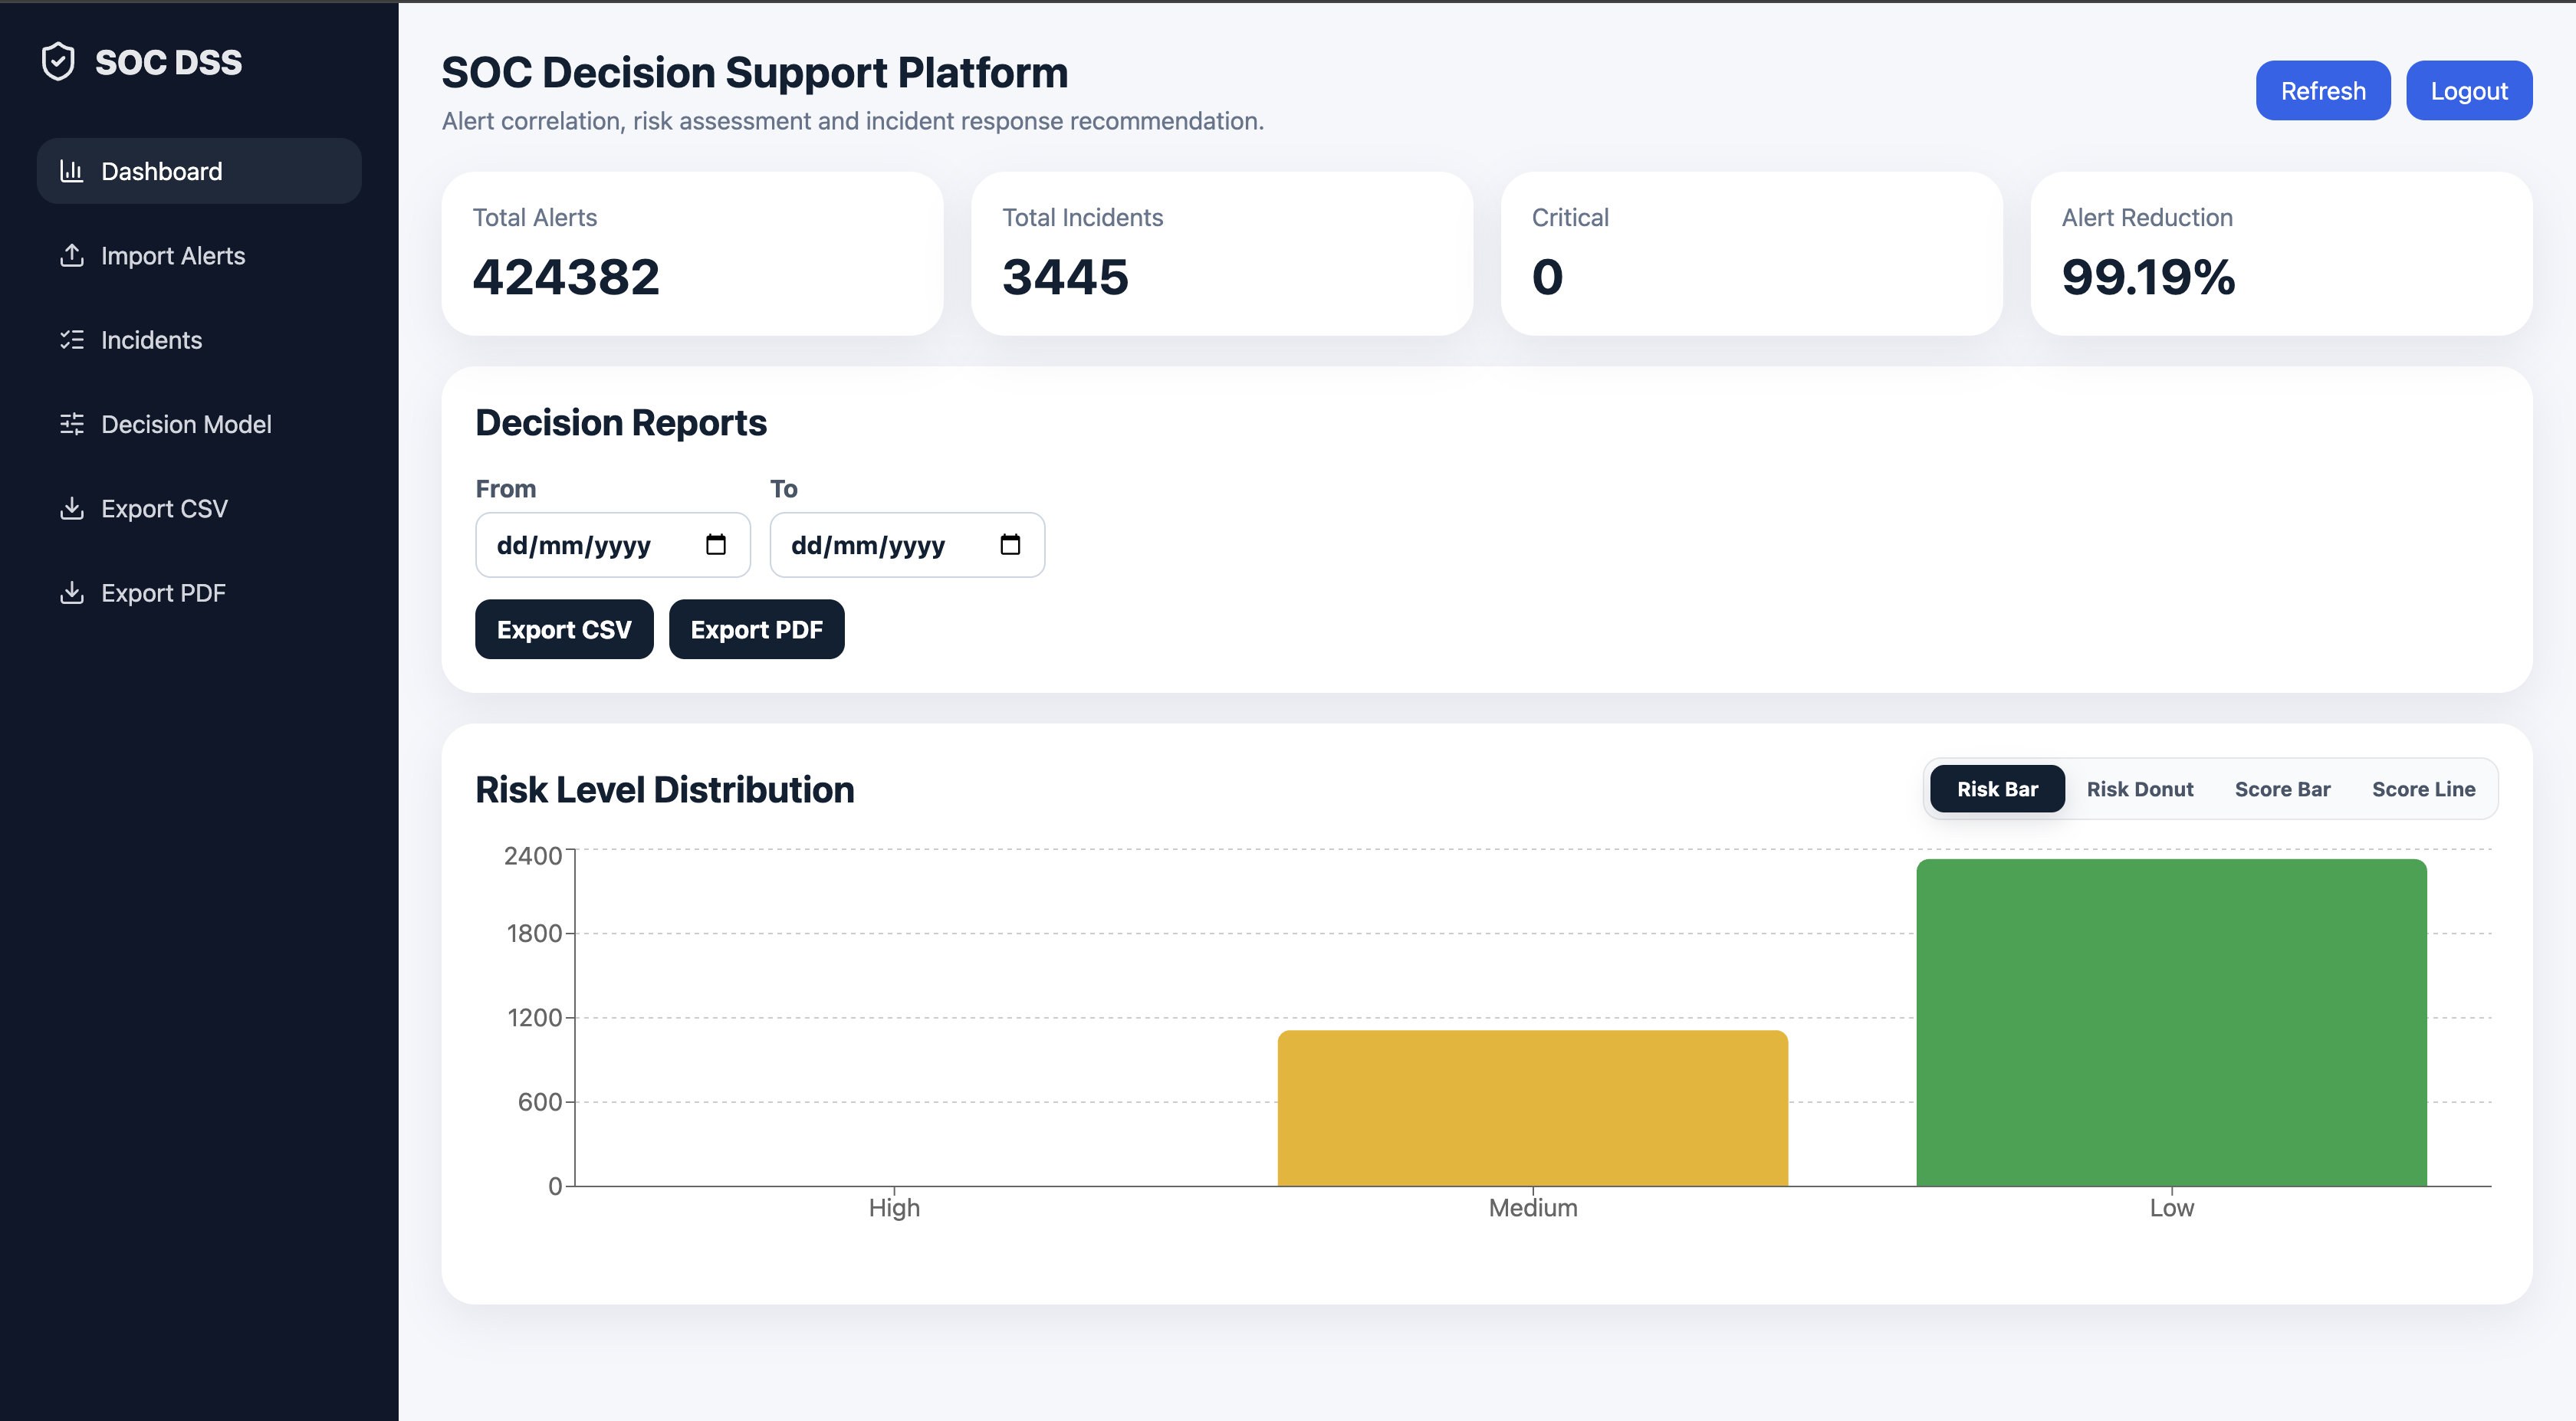
\includegraphics[width=\textwidth]{images/do_thi_incident.png}
    \caption{Dashboard tổng quan và phân bố mức rủi ro của incident sau tương quan}
    \label{fig:dashboard-risk-distribution}
\end{figure}

}

\section{Kịch bản thực nghiệm}
{\fontsize{13pt}{15.6pt}\selectfont

Đề tài sử dụng ba nhóm kịch bản thực nghiệm. Nhóm thứ nhất là kịch bản import log lớn nhằm đánh giá khả năng tiếp nhận dữ liệu thực tế và tránh lỗi giới hạn kích thước request. Nhóm thứ hai là kịch bản correlation trên toàn bộ tập alert đã import nhằm đo tỷ lệ giảm cảnh báo sau khi gom nhóm. Nhóm thứ ba là kịch bản đánh giá đầu ra DSS, bao gồm phân bố risk level, decision advice và khả năng export báo cáo theo khoảng ngày.

\begingroup\small
\begin{longtable}{|L{3.2cm}|L{4.5cm}|L{5.8cm}|}
\hline
\textbf{Kịch bản} & \textbf{Nguồn dữ liệu} & \textbf{Mục tiêu đánh giá} \\
\hline
\endfirsthead
\hline
\textbf{Kịch bản} & \textbf{Nguồn dữ liệu} & \textbf{Mục tiêu đánh giá} \\
\hline
\endhead
Large log import & Wazuh/AMiner JSON-lines kích thước lớn & Đánh giá khả năng chia batch upload, import dữ liệu lớn và tránh lỗi giới hạn kích thước request. \\
\hline
Correlation toàn bộ dữ liệu & 74.517 cảnh báo đã import & Đánh giá khả năng gom nhóm alert thành incident và đo tỷ lệ giảm cảnh báo. \\
\hline
Risk distribution & 3.445 incident sau correlation & Đánh giá phân bố mức rủi ro và khả năng ưu tiên sự cố. \\
\hline
Report export & Incident đã tương quan trong database & Đánh giá khả năng xuất CSV/PDF theo khoảng ngày phục vụ báo cáo học thuật và vận hành. \\
\hline
\caption{Các kịch bản thực nghiệm của hệ thống}\\
\end{longtable}
\endgroup

}

\section{Chỉ số đánh giá}
{\fontsize{13pt}{15.6pt}\selectfont

Các chỉ số đánh giá được lựa chọn dựa trên mục tiêu của hệ hỗ trợ quyết định:

\begin{itemize}
    \item \textbf{Số lượng raw alerts:} tổng số cảnh báo đầu vào được import.
    \item \textbf{Số lượng correlated incidents:} số incident sau khi gom nhóm.
    \item \textbf{Alert reduction rate:} tỷ lệ giảm đơn vị cần xử lý, tính theo công thức:
    \[
    \mathrm{Reduction} = \frac{\mathrm{RawAlerts} - \mathrm{Incidents}}{\mathrm{RawAlerts}} \times 100\%
    \]
    \item \textbf{Risk score và risk level:} điểm và mức rủi ro của từng incident.
    \item \textbf{Decision priority:} mức ưu tiên P1--P4 do DSS sinh ra.
    \item \textbf{Recommendation quality:} mức độ phù hợp và khả năng hành động của khuyến nghị.
\end{itemize}

}

\section{Kết quả tương quan cảnh báo}
{\fontsize{13pt}{15.6pt}\selectfont

Kết quả trên phiên thực nghiệm dữ liệu lớn cho thấy hệ thống có thể giảm số lượng đơn vị cần xử lý từ 74.517 raw alerts xuống 3.445 incidents. Tỷ lệ giảm cảnh báo đạt 95,38\%. Kết quả này cho thấy module correlation có khả năng gom các cảnh báo có cùng ngữ cảnh thành incident ở mức cao hơn, qua đó giảm đáng kể khối lượng triage thủ công cho SOC analyst.

\begin{longtable}{|L{4.0cm}|C{2.6cm}|C{3.3cm}|C{2.5cm}|}
\hline
\textbf{Kịch bản} & \textbf{Raw alerts} & \textbf{Correlated incidents} & \textbf{Reduction} \\
\hline
\endfirsthead
\hline
\textbf{Kịch bản} & \textbf{Raw alerts} & \textbf{Correlated incidents} & \textbf{Reduction} \\
\hline
\endhead
Phiên thực nghiệm dữ liệu lớn & 74.517 & 3.445 & 95,38\% \\
\hline
\caption{Kết quả tương quan cảnh báo trên các kịch bản thực nghiệm}\label{tab:correlation-results}\\
\end{longtable}

\noindent Tỷ lệ giảm 95,38\% có ý nghĩa thực tiễn đối với vận hành SOC. Thay vì buộc analyst đọc toàn bộ 74.517 alert riêng lẻ, hệ thống chuyển dữ liệu đầu vào thành 3.445 incident có ngữ cảnh, điểm rủi ro và khuyến nghị phản ứng. Điều này không loại bỏ vai trò kiểm chứng của con người, nhưng giúp chuyển trọng tâm xử lý từ raw log sang các đơn vị sự cố có ý nghĩa hơn.

}

\section{Kết quả đánh giá rủi ro}
{\fontsize{13pt}{15.6pt}\selectfont

Sau khi tương quan, mỗi incident được tính risk score theo mô hình đã đề xuất. Kết quả dashboard của phiên thực nghiệm ghi nhận 0 incident Critical và không quan sát thấy cột High trong biểu đồ phân bố. Phần lớn incident nằm ở mức Low, một phần đáng kể ở mức Medium. Phân bố này cho thấy hệ thống không mặc định gán tất cả incident ở mức cao, mà phân biệt theo severity, tần suất và ngữ cảnh tài sản.

\begingroup\small
\begin{longtable}{|L{2.5cm}|C{2.2cm}|L{4.1cm}|L{3.8cm}|}
\hline
\textbf{Mức rủi ro} & \textbf{Số lượng quan sát} & \textbf{Diễn giải} & \textbf{Ý nghĩa đối với triage} \\
\hline
\endfirsthead
\hline
\textbf{Mức rủi ro} & \textbf{Số lượng quan sát} & \textbf{Diễn giải} & \textbf{Ý nghĩa đối với triage} \\
\hline
\endhead
Critical & 0 & Không có incident vượt ngưỡng rủi ro nghiêm trọng nhất trong phiên chạy. & Không phát sinh nhóm cần escalation khẩn cấp theo ngưỡng Critical. \\
\hline
High & 0 theo biểu đồ & Không quan sát thấy cột High trong phiên thực nghiệm. & Không có nhóm P2 nổi bật cần xử lý trước Medium/Low. \\
\hline
Medium & Xấp xỉ 1,1 nghìn incident & Nhóm incident có điểm rủi ro trung bình, thấp hơn ngưỡng High/Critical. & Cần xác minh, theo dõi và ưu tiên sau các incident nghiêm trọng. \\
\hline
Low & Xấp xỉ 2,3 nghìn incident & Nhóm incident chiếm đa số trong tổng 3.445 incident. & Phù hợp đưa vào hàng đợi triage thông thường hoặc xử lý theo batch. \\
\hline
\caption{Tóm tắt kết quả đánh giá rủi ro trên dashboard thực nghiệm}\\
\end{longtable}
\endgroup

\noindent Về mặt đánh giá, kết quả phân bố rủi ro cho thấy mô hình risk scoring đóng vai trò lọc và phân tầng incident sau correlation. Các incident mức Low chiếm đa số, trong khi nhóm Medium vẫn cần được analyst theo dõi để phát hiện các dấu hiệu leo thang. Việc không xuất hiện Critical trong phiên thực nghiệm không phải là hạn chế của mô hình, mà phản ánh rằng dữ liệu nhập vào chưa tạo ra incident vượt ngưỡng nghiêm trọng nhất theo cấu hình risk model hiện tại.

}

\section{Kết quả hỗ trợ quyết định và khuyến nghị phản ứng}
{\fontsize{13pt}{15.6pt}\selectfont

Module decision support chuyển risk level thành priority và hành động có thể thực hiện. Với incident Critical hoặc score từ 85 trở lên, hệ thống sinh priority P1, SLA 1 giờ và khuyến nghị escalation ngay cho nhóm L2 incident response. Với incident High, hệ thống thường sinh P2, SLA 4 giờ và khuyến nghị xác minh hoạt động độc hại trước khi containment.

\begingroup\small
\begin{longtable}{|L{3.0cm}|C{1.6cm}|C{1.8cm}|L{7.1cm}|}
\hline
\textbf{Incident} & \textbf{Priority} & \textbf{SLA} & \textbf{Khuyến nghị phản ứng} \\
\hline
\endfirsthead
\hline
\textbf{Incident} & \textbf{Priority} & \textbf{SLA} & \textbf{Khuyến nghị phản ứng} \\
\hline
\endhead
SSH Brute Force & P1 & 1 giờ & Chặn source IP nếu xác minh tấn công, kiểm tra đăng nhập thành công, rà soát privilege escalation và lưu bằng chứng. \\
\hline
FIM File Change & P2 & 4 giờ & Xác minh thay đổi tệp, đối chiếu change request, thu thập log và cô lập host nếu có dấu hiệu compromise. \\
\hline
Vulnerability Incident & P2/P3 & 4--24 giờ & Tạo remediation ticket, ưu tiên vá lỗi theo tài sản và mức exposure, theo dõi SLA xử lý. \\
\hline
General Alert & P4 & 72 giờ & Đưa vào hàng đợi L1 triage, tiếp tục theo dõi và ghi nhận analyst verdict. \\
\hline
\caption{Ví dụ kết quả hỗ trợ quyết định}\\
\end{longtable}
\endgroup

\noindent Kết quả này phù hợp với vai trò của DSS: không tự động thực thi hành động nguy hiểm trên production, mà đưa ra khuyến nghị, SLA và lý do để analyst quyết định. Đặc biệt, trường \texttt{rationale} giúp analyst hiểu vì sao hệ thống gán incident vào một priority cụ thể.

\begin{figure}[H]
    \centering
    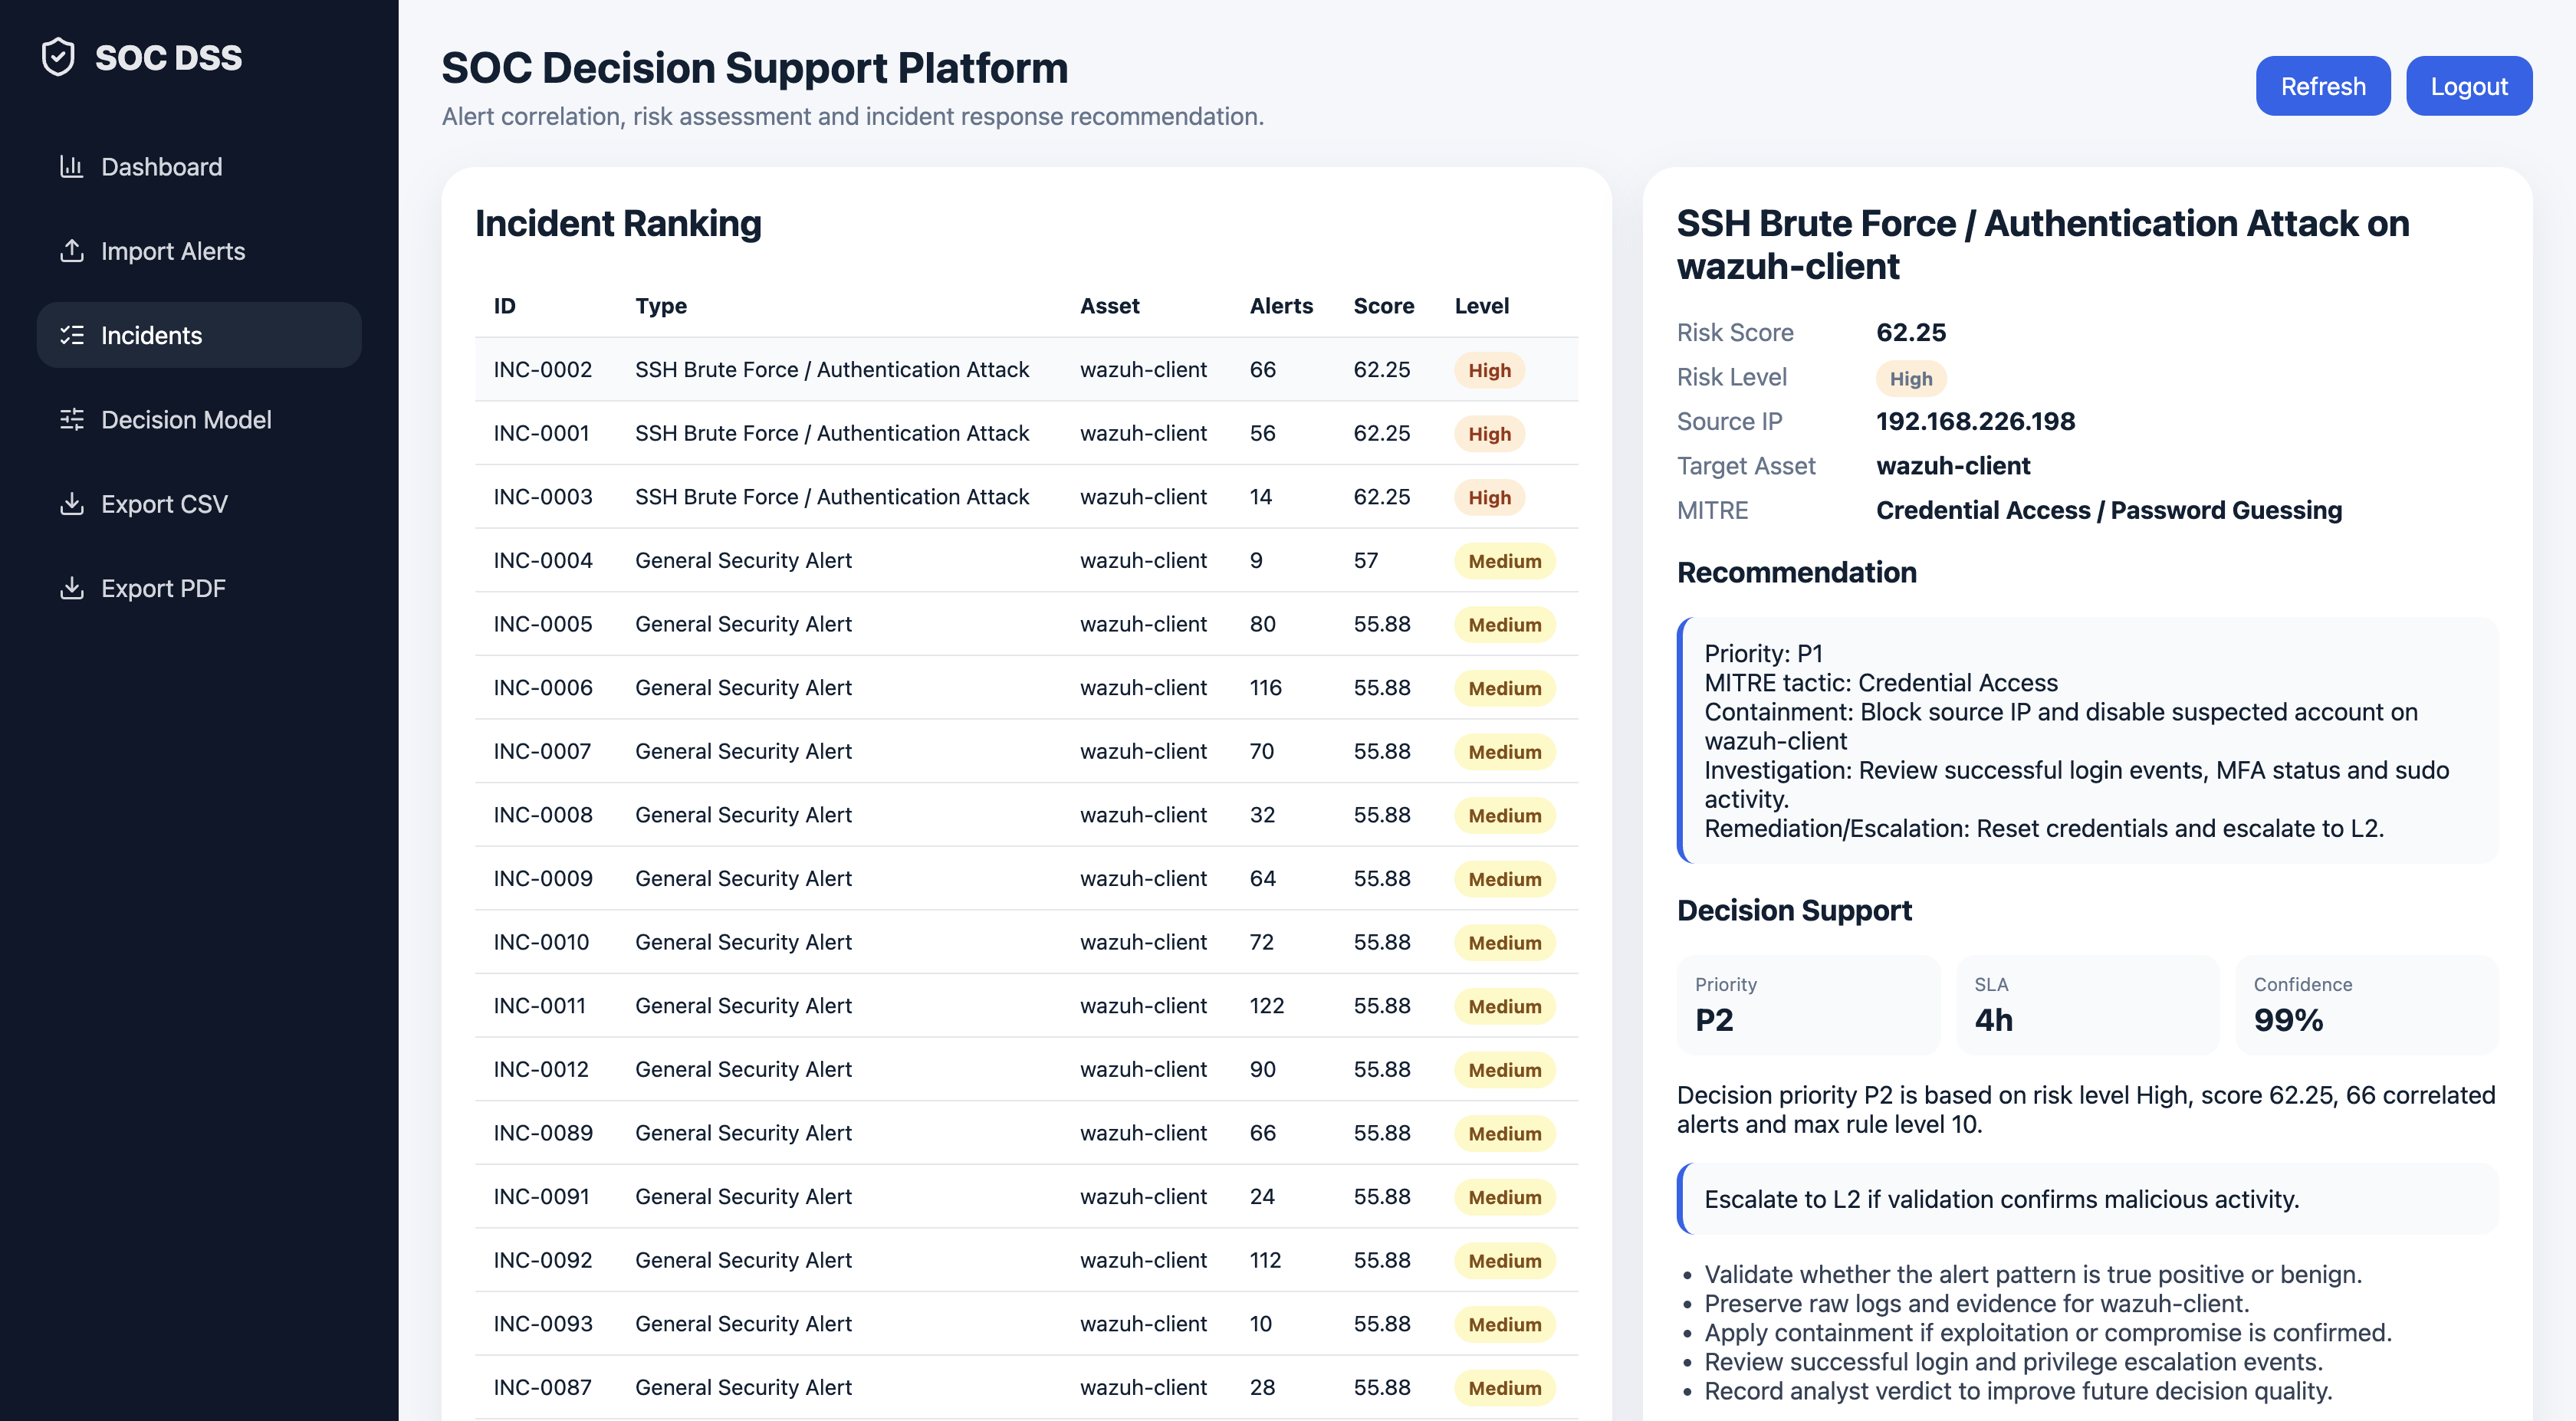
\includegraphics[width=\textwidth]{images/incident.png}
    \caption{Màn hình xếp hạng incident và chi tiết khuyến nghị hỗ trợ quyết định}
    \label{fig:incident-ranking-decision-support}
\end{figure}

}

\section{Đánh giá chức năng báo cáo}
{\fontsize{13pt}{15.6pt}\selectfont

Chức năng báo cáo hỗ trợ xuất dữ liệu incident theo khoảng ngày tùy chọn. Báo cáo CSV phù hợp cho phân tích định lượng và xử lý bằng công cụ bảng tính; báo cáo PDF phù hợp cho trình bày kết quả cho giảng viên, quản lý hoặc nhóm vận hành. Việc cho phép chọn \texttt{from} và \texttt{to} giúp người nghiên cứu tách riêng từng phiên thực nghiệm, tránh phụ thuộc vào các khoảng cố định như tuần, tháng hoặc năm.

\noindent Nội dung báo cáo gồm các trường quan trọng: incident ID, title, incident type, source IP, target asset, alert count, max rule level, risk score, risk level, decision priority, SLA, confidence, escalation, analyst verdict, decision status và recommendation. Như vậy, báo cáo không chỉ phản ánh dữ liệu thô mà còn thể hiện kết quả xử lý của DSS.

}

\section{Thảo luận kết quả}
{\fontsize{13pt}{15.6pt}\selectfont

Kết quả thực nghiệm cho thấy hệ hỗ trợ quyết định đề xuất đáp ứng được các mục tiêu chính của đề tài. Thứ nhất, hệ thống có khả năng giảm số lượng cảnh báo cần xử lý thông qua correlation, thể hiện qua kết quả 74.517 alert được gom thành 3.445 incident. Thứ hai, mô hình risk scoring giúp phân biệt mức ưu tiên dựa trên nhiều yếu tố ngữ cảnh thay vì chỉ dựa vào rule level. Thứ ba, module decision support biến điểm rủi ro thành priority, SLA và hành động khuyến nghị, qua đó hỗ trợ trực tiếp cho quy trình triage trong SOC.

\noindent Tuy nhiên, kết quả cũng cần được nhìn nhận trong phạm vi giới hạn. Tỷ lệ giảm cảnh báo cho thấy hệ thống có khả năng chuyển đổi raw alert thành incident ở mức cao hơn, nhưng chưa thể hiện đầy đủ mức cải thiện về hiệu quả vận hành nếu so sánh với quy trình analyst thao tác trực tiếp trên giao diện mặc định của Wazuh hoặc một SIEM/XDR khác. Do đó, kết quả hiện tại phù hợp để chứng minh tính khả thi của hướng tiếp cận, trong khi các nghiên cứu tiếp theo cần bổ sung baseline comparison để đo các chỉ số như thời gian triage, số lượng alert cần đọc, mức độ chính xác khi ưu tiên sự cố và mức độ nhất quán giữa các analyst.

\noindent Ngoài ra, mô hình risk scoring hiện sử dụng các trọng số tĩnh do người thiết kế xác định dựa trên lập luận nghiệp vụ và yêu cầu giải thích của DSS. Cách tiếp cận này phù hợp với giai đoạn prototype, nhưng chưa tương đương với việc định lượng trọng số bằng các phương pháp ra quyết định đa tiêu chí như AHP, Delphi hoặc đánh giá chuyên gia nhiều vòng. Vì vậy, risk score trong phiên bản hiện tại nên được hiểu là cơ chế xếp hạng có khả năng giải thích, không phải là thước đo rủi ro đã được tối ưu hóa cho mọi môi trường SOC.

\noindent Một giới hạn quan trọng khác là tập dữ liệu thực nghiệm chưa có ground truth đầy đủ. Khi chưa có nhãn chuẩn cho từng alert, incident và mức rủi ro thực tế, hệ thống chưa thể được đánh giá bằng các chỉ số như precision, recall hoặc F1-score đối với kết quả correlation và risk classification. Vì vậy, kết quả hiện tại chứng minh giá trị hỗ trợ quyết định và khả năng giảm tải alert, nhưng chưa khẳng định độ chính xác tuyệt đối của mô hình trong mọi kịch bản tấn công.


}

\chapter{\MakeTextUppercase{Kết luận và hướng phát triển}}

\section{Kết luận}
{\fontsize{13pt}{15.6pt}\selectfont

Đề tài đã nghiên cứu và xây dựng một hệ hỗ trợ quyết định cho tương quan cảnh báo, đánh giá rủi ro và hỗ trợ phản ứng sự cố an toàn thông tin trong môi trường SOC. Trên cơ sở lý thuyết về DSS, SOC, alert correlation, risk assessment, incident response và MITRE ATT\&CK, đề tài đã đề xuất một mô hình tích hợp gồm các bước: tiếp nhận cảnh báo, chuẩn hóa dữ liệu, phân loại cảnh báo, tương quan thành incident, đánh giá rủi ro và đề xuất phản ứng.

\noindent Prototype của đề tài đã hiện thực hóa mô hình đề xuất bằng backend Spring Boot, frontend React/TypeScript, PostgreSQL và Docker Compose. Hệ thống hỗ trợ import Wazuh/AMiner logs, xử lý file lớn theo batch, correlation bất đồng bộ, dashboard risk visualization, decision model, analyst feedback, xác thực đăng nhập và export báo cáo CSV/PDF theo khoảng ngày tùy chọn.

\noindent Kết quả thực nghiệm trên phiên xử lý dữ liệu lớn cho thấy hệ thống có thể giảm 74.517 raw alerts xuống 3.445 incidents, tương ứng tỷ lệ giảm cảnh báo 95,38\%. Dashboard thực nghiệm ghi nhận 0 incident Critical và phân bố incident chủ yếu ở Low, một phần ở Medium. Mô hình risk scoring và decision advice giúp chuyển đổi cảnh báo kỹ thuật thành thông tin hỗ trợ quyết định như risk level, priority, SLA, escalation và next actions.

}

\section{Đóng góp đạt được}
{\fontsize{13pt}{15.6pt}\selectfont

Các kết quả chính của đề tài gồm:

\begin{itemize}
    \item Xây dựng được mô hình DSS tích hợp cho môi trường SOC, kết hợp correlation, risk assessment và incident response recommendation.
    \item Hiện thực được prototype hệ hỗ trợ quyết định có khả năng chạy end-to-end từ import alert đến dashboard và export report.
    \item Đề xuất được mô hình risk scoring có tính giải thích, dựa trên severity, asset criticality, frequency, MITRE context, exposure và vulnerability context.
    \item Xây dựng được cơ chế decision advice gồm priority, SLA, confidence, escalation và next actions.
    \item Bổ sung chức năng analyst feedback và report export, tạo cơ sở cho đánh giá học thuật và vận hành SOC.
\end{itemize}

}

\section{Hạn chế}
{\fontsize{13pt}{15.6pt}\selectfont

Mặc dù đạt được mục tiêu đề ra, hệ thống vẫn tồn tại một số hạn chế. Thứ nhất, phần thực nghiệm chưa có baseline comparison với quy trình xử lý cảnh báo trực tiếp trên Wazuh hoặc một nền tảng SIEM/XDR mặc định. Vì vậy, báo cáo mới chứng minh được tỷ lệ giảm số lượng alert sau correlation, nhưng chưa đo định lượng mức cải thiện về thời gian xử lý, khối lượng thao tác và chất lượng quyết định của analyst.

\noindent Thứ hai, mô hình risk scoring sử dụng các trọng số tĩnh do người thiết kế xác định. Các trọng số này giúp mô hình dễ giải thích và phù hợp với prototype nghiên cứu, nhưng chưa được hiệu chỉnh bằng các phương pháp khoa học như AHP, Delphi, đánh giá chuyên gia nhiều vòng hoặc học từ dữ liệu lịch sử vận hành SOC.

\noindent Thứ ba, tập dữ liệu thực nghiệm chưa có ground truth đầy đủ. Do đó, hệ thống chưa thể đánh giá chính xác precision/recall của việc gom nhóm alert thành incident, cũng như chưa đo được tỷ lệ incident bị phân loại sai mức rủi ro. Đây là hạn chế quan trọng nếu muốn khẳng định độ chính xác của mô hình trên dữ liệu thực tế.

\noindent Thứ tư, mô hình correlation hiện tại chủ yếu dựa trên rule và khóa nhóm đơn giản, nên chưa phát hiện đầy đủ các chuỗi tấn công phức tạp nhiều giai đoạn. Module recommendation cũng mới dừng ở khuyến nghị bán tự động, chưa tích hợp trực tiếp với SOAR, ticketing system hoặc active response.

}

\section{Hướng phát triển}
{\fontsize{13pt}{15.6pt}\selectfont

Trong các nghiên cứu và phiên bản tiếp theo, hệ thống có thể được phát triển theo các hướng sau:

\begin{itemize}
    \item Mở rộng tích hợp trực tiếp với Wazuh Indexer API hoặc SIEM/XDR khác để thu thập cảnh báo gần thời gian thực.
    \item Bổ sung correlation theo attack chain, MITRE ATT\&CK tactic sequence và graph-based correlation.
    \item Hiệu chỉnh mô hình risk scoring bằng dữ liệu lịch sử, phản hồi analyst và phương pháp học máy có khả năng giải thích.
    \item Tích hợp MITRE D3FEND để ánh xạ kỹ thuật tấn công sang biện pháp phòng thủ cụ thể.
    \item Tích hợp SOAR hoặc ticketing system để tự động tạo ticket, theo dõi SLA và bán tự động hóa một số hành động phản ứng.
    \item Xây dựng bộ benchmark lớn hơn với nhiều nguồn dữ liệu như Wazuh, AMiner, IDS, firewall và endpoint telemetry.
    \item Hoàn thiện cơ chế phân quyền nhiều người dùng, audit log và quản trị cấu hình cho môi trường production.
\end{itemize}

}

\section{Kết luận chung}
{\fontsize{13pt}{15.6pt}\selectfont

Từ các kết quả đã đạt được, có thể khẳng định rằng hướng tiếp cận DSS cho môi trường SOC là phù hợp và có tính ứng dụng thực tiễn. Việc kết hợp tương quan cảnh báo, đánh giá rủi ro theo ngữ cảnh và khuyến nghị phản ứng giúp chuyển đổi dữ liệu cảnh báo rời rạc thành thông tin hỗ trợ quyết định có giá trị. Prototype hiện thực trong đề tài vì vậy có thể được sử dụng phục vụ nghiên cứu, giảng dạy và minh họa quy trình hỗ trợ quyết định trong hoạt động giám sát an toàn thông tin.

}

\clearpage
\thispagestyle{empty}
\phantomsection
\addcontentsline{toc}{chapter}{\MakeTextUppercase{Tài liệu tham khảo}}

\vspace{0.6cm}

\nocite{*}
\bibliographystyle{IEEEtran}
\bibliography{references}

\end{document}